\chapter{Dispositivi MOSFET}
\section{Cos'è il condensatore MOS}
Partiamo dal nome:
\begin{itemize}
    \item MOS: Metal–Oxide–Semiconductor
    \item FET: field–effect transistor
\end{itemize}
ovvero transistore metallo-ossido-semiconduttore ad effetto di campo, questo dispositivo è alla	base	dei	circuiti	a	MOSFET.

\section{Come è fatto}
Costituito	da	un	layer conduttore	detto	\textbf{gate},	separato	da	un	
substrato in	silicio	drogato	(di	tipo	p	o	n) e	da	uno	strato	isolante
di	biossido	di	silicio ($SiO_2$), utilizzato	per	indurre	una	carica	superficiale	all'interfaccia	tra	il	
silicio	e	il	biossido	di	silicio.

\begin{figure}[htbp]
    \centering
    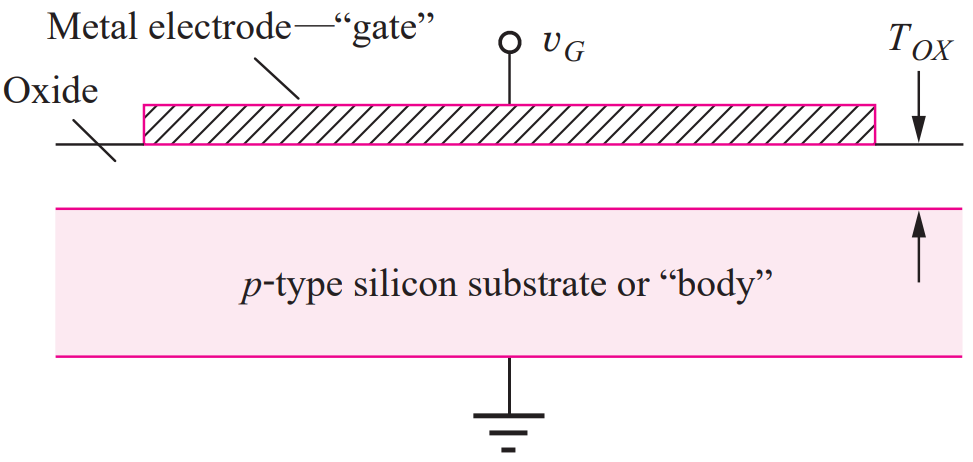
\includegraphics[width=0.4\linewidth]{img/cond_mos.png}
    \caption{Condensatore MOSFET}    
\end{figure}

Ricorda proprio un condensatore a piatti, tranne che al posto di esserci un metallo da entrambe le facce troviamo un semiconduttore e un metallo, dunque alteriamo le normali caratteristiche di un condensatore.

\subsection{Regione	di	accumulazione}
La polarizzazione negativa avviene quando sul gate troviamo cariche negative, mentre sotto al gate troviamo cariche positive composta da lacune.

Dunque si dice che la superficie	del	semiconduttore	è	in	accumulo. Sostanzialmente abbiamo accumulato le cariche presenti nel substrato drogato di silicio sulla sua superficie.

\begin{figure}[htbp]
    \centering
    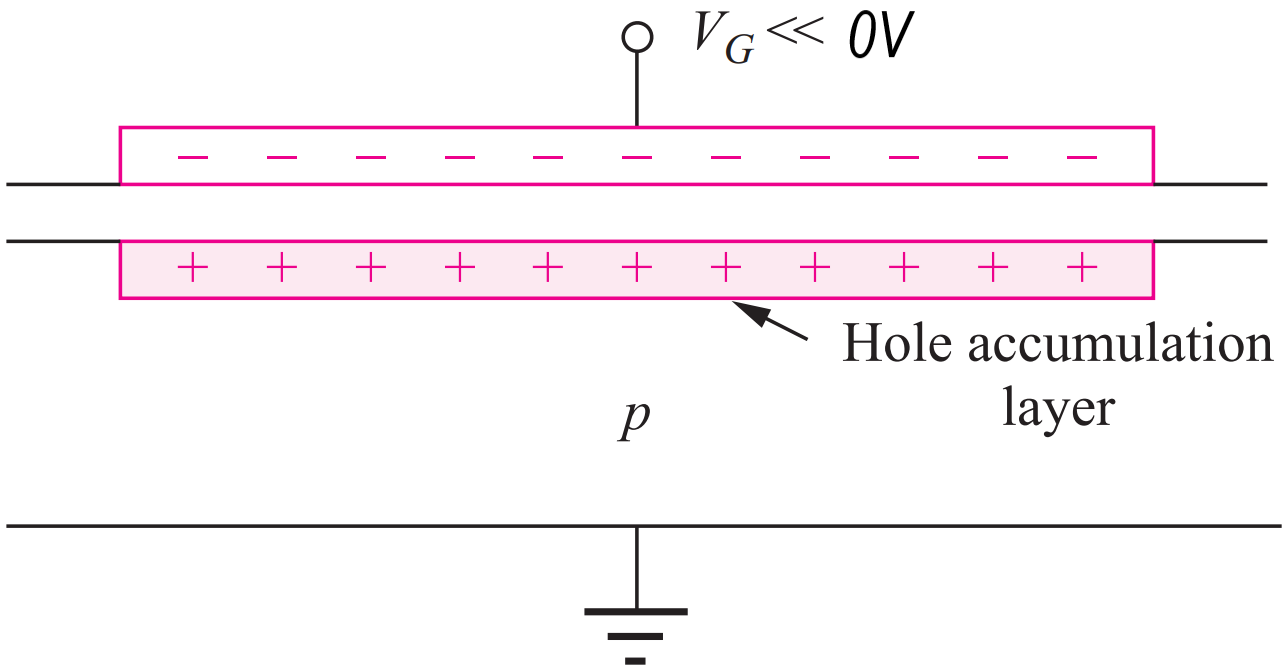
\includegraphics[width=0.4\linewidth]{img/polarizza_neg.png}  
    \caption{Regione	di	accumulazione}   
\end{figure}

\newpage
\subsection{Regione	di	svuotamento}
Il	potenziale	del	gate	viene	incrementato	(>	0V). Dunque il campo elettrico è diretto verso il basso e allontana le lacune dalla superficie. Allontana le lacune ma rimangono gli ioni negativi degli atomi accettori che abbiamo utilizzato per produrre il substrato di tipo p, i quali controbilanceranno la carica positiva che si è formata sul gate.

Dunque ecco perché il nome zona di svuotamento, perché abbiamo allontanato, svuotato, la zona dalle lacune.

Da notare che gli ioni nel substrato sono \textbf{fissi} perché fanno parte del reticolo cristallino del silicio.

\begin{figure}[htbp]
    \centering
    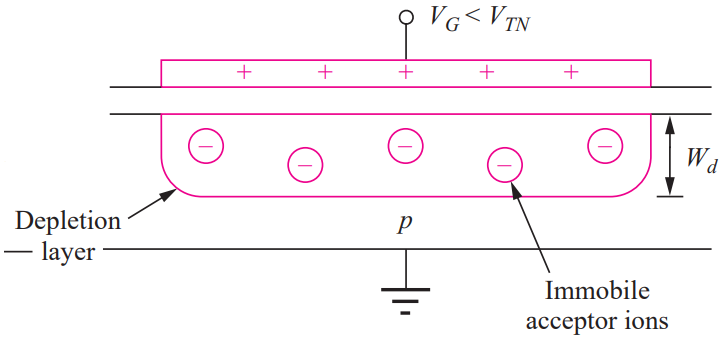
\includegraphics[width=0.47\linewidth]{img/regione_svuotmamnto.png}
    \caption{Regione	di	svuotamento}    
\end{figure}

\subsection{Regione	di	inversione}
Se aumentiamo ancora la tensione sul gate, gli elettroni sono attratti sulla superficie del substrato, dunque la carica positiva nel metallo ora viene bilanciata dagli ioni fissi e da elettroni nel substrato.
\paragraph{}
Quando il numero di elettroni supera il numero di lacune, ci troviamo in condizione della cosiddetta \textbf{inversione}. La tensione alla quale si forma lo strato	di	inversione	è	chiamata	
\textbf{tensione	di	soglia},	indicata	con	VT (o	VTN per	gli	elettroni).



\begin{figure}[htbp]
    \centering
    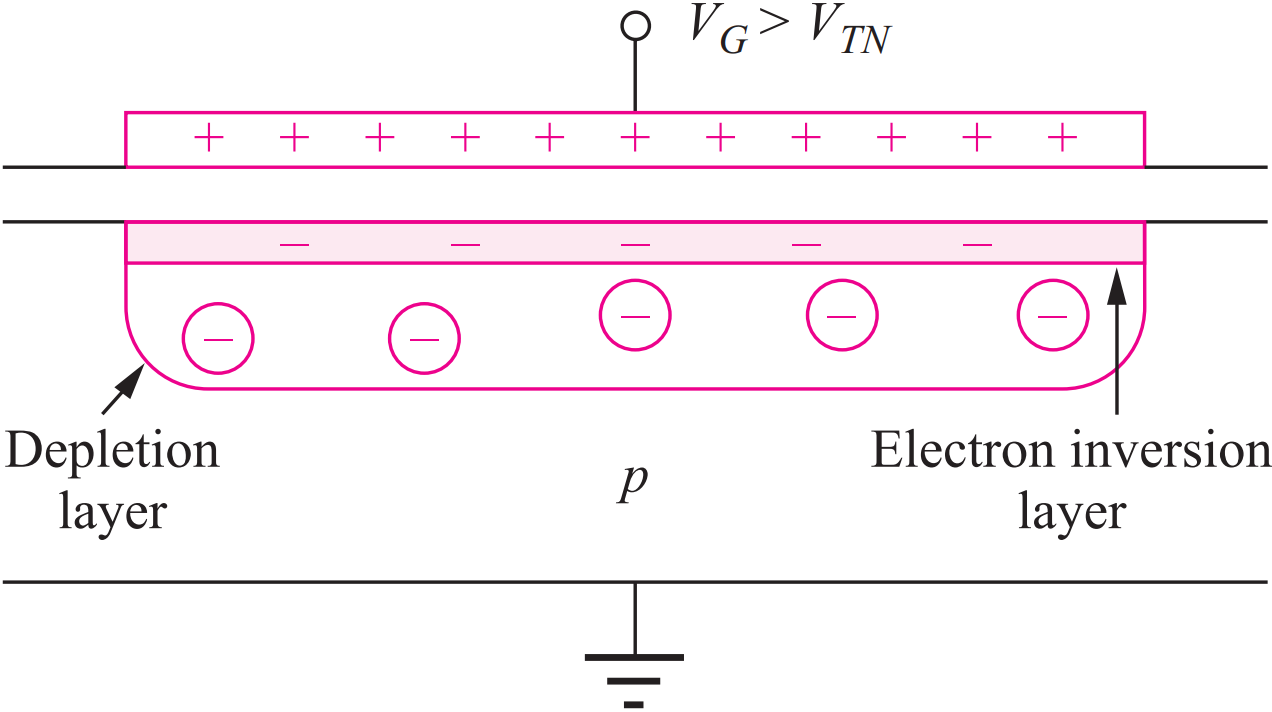
\includegraphics[width=0.4\linewidth]{img/inversione.png}
    \caption{Regione	di	inversione}
    
\end{figure}

Dunque è come se avessimo fatto uno strato di tipo n sopra le lacune del substrato, abbiamo creato uno \textbf{strato conduttore}, praticamente fatto a comando variando la tensione sul gate, che mette in contatto il lato destro e sinistro del condensatore.

Ci fa comodo questo strato, infatti ai lati possiamo mettere due terminali ed otteniamo appunto il \textbf{transistore}.

\newpage
\section{Il transistore nMOS}

Ai lati del gate, mettiamo due regioni di tipo n+ (tanti elettroni) chiamati: \textbf{source}  e \textbf{drain}.

Questi due terminali sono messi in modo tale che possano mettersi in contatto con lo strato di inversione discusso in precedenza, formando di fatto una sorta di U rovesciata.


\begin{figure}[htbp]
    \centering
    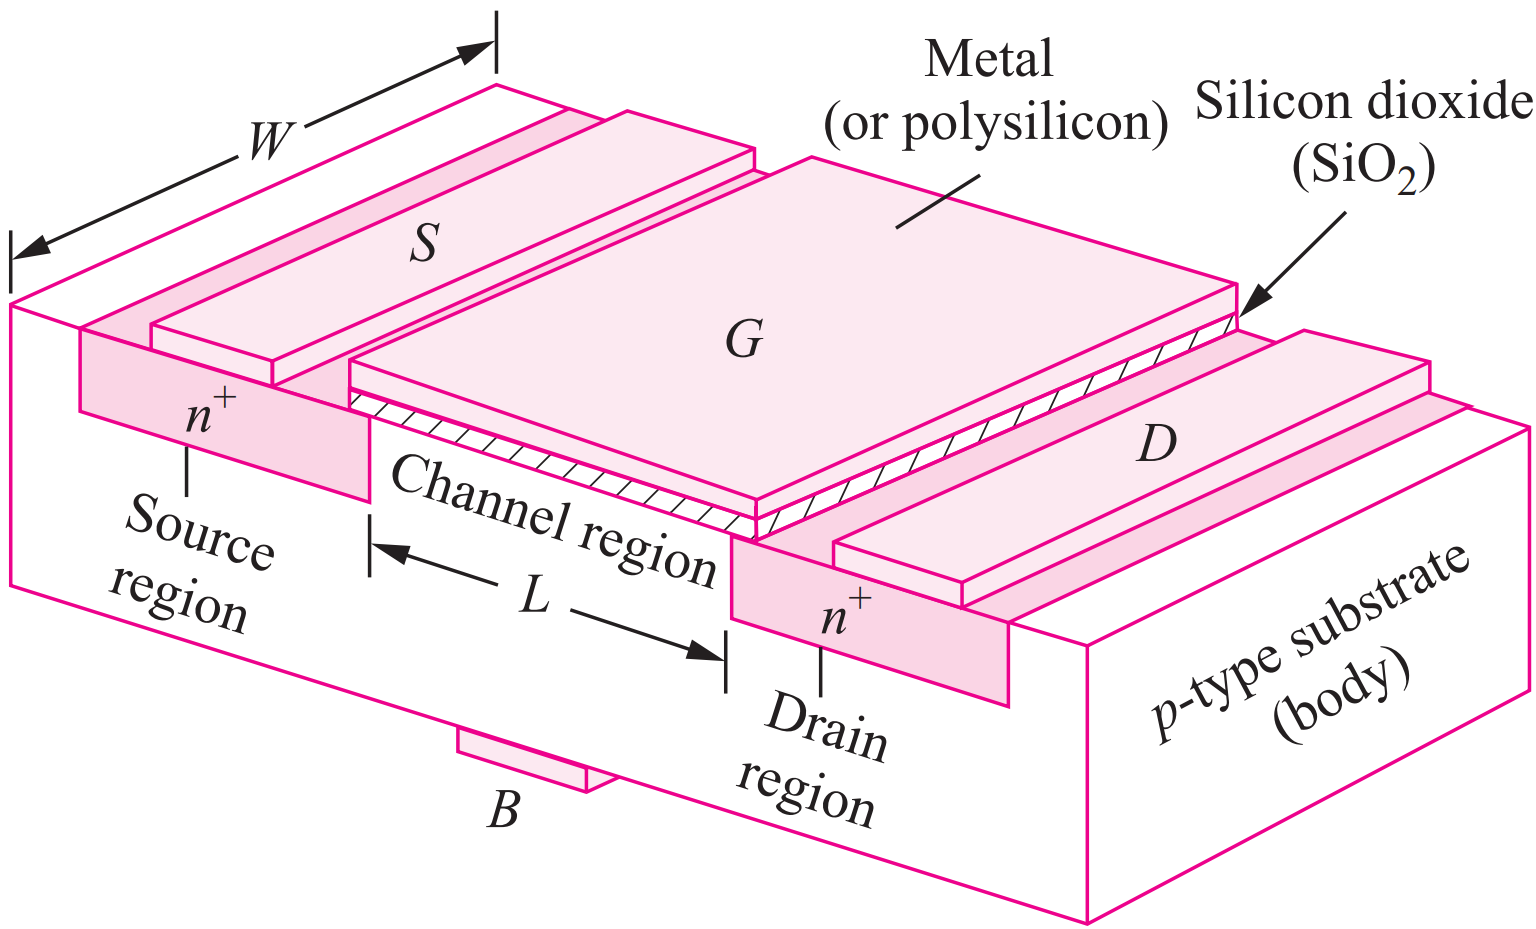
\includegraphics[width=0.5\linewidth]{img/nMOS.png}
    \caption{Transistore nMOS}    
\end{figure}

Il transistore ha due parametri molto importanti che influenzano le caratteristiche elettrice del circuito:
\begin{itemize}
    \item Distanza tra i terminali, lunghezza L del canale;
    \item Larghezza del transistore
\end{itemize}

Con più la lunghezza è piccola più il costo per stampare il circuito diventerà costoso $\approx 10nm$. Questa tipologia di transistori veniva più utilizzata una decina di anni fa, ora si è passati ad un nuovo transistore chiamato \textbf{FinFET} tridimensionale e non più planare, consentendo ulteriormente la miniaturizzazione.

\subsection{Simbolo circuitale}
Le zone di source e drain sono terminali fortemente drogate con atomi donatori, e possono anche essi donare elettroni per formare lo strato di inversione.
Le stesse regioni formano anche due diodi con il substrato (giunzione p-n), i quali sono normalmente \textbf{polarizzati inversamente}, in prima approssimazione è come se non ci fossero. Creano solo una carica spaziale introno alle due connessioni.

\begin{figure}[htbp]
    \centering
    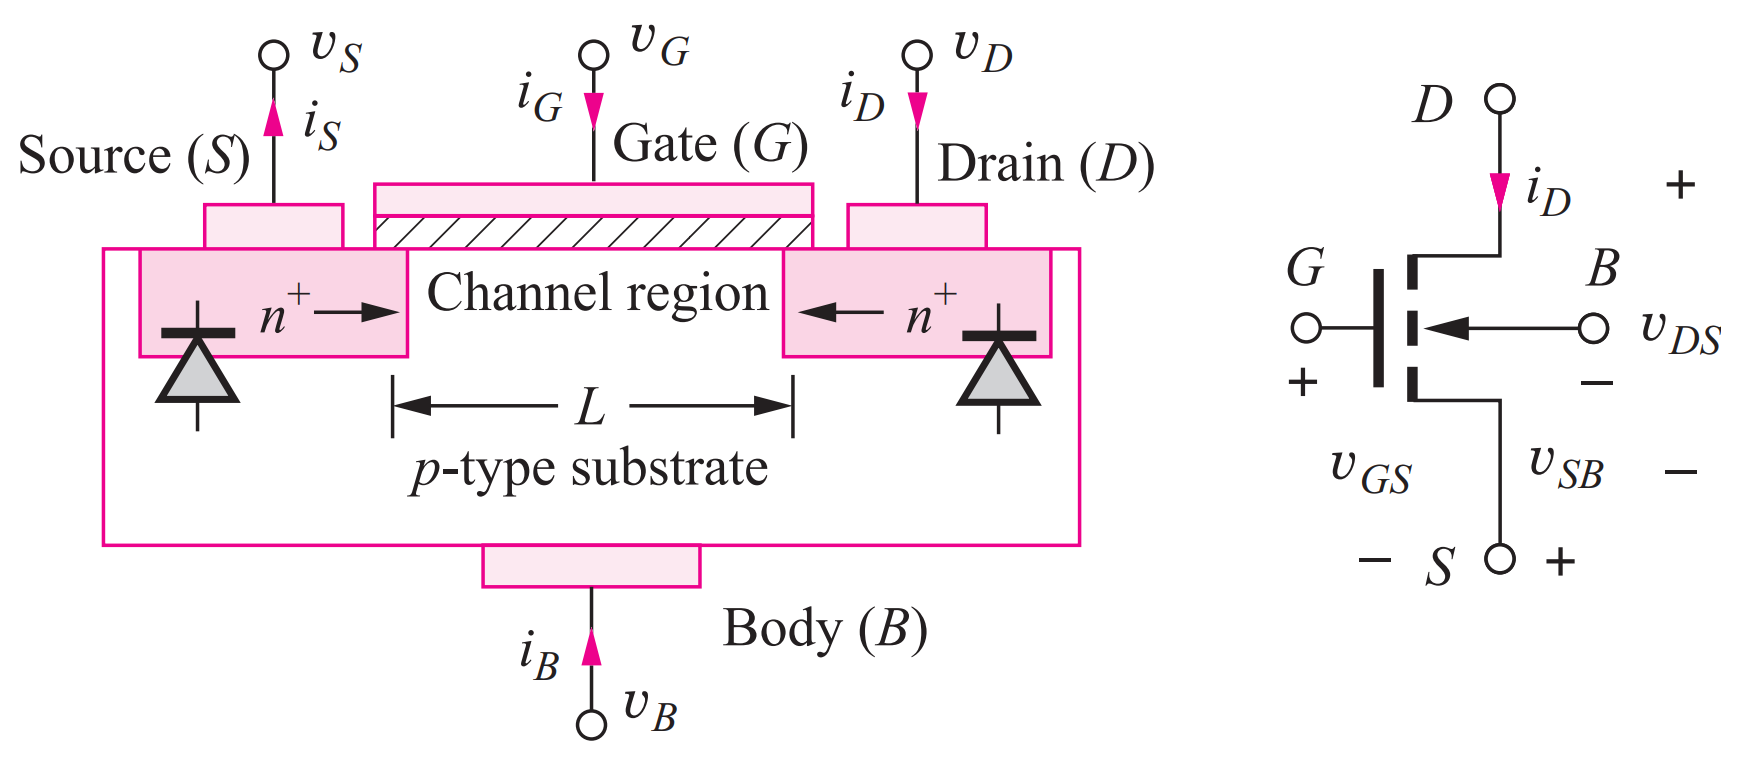
\includegraphics[width=0.65\linewidth]{img/nMoas.png}
    \caption{Transistore nMOS}
    
\end{figure}

\subsection{Funzionamento qualitativo}

Assumiamo ora di mettere $V_B = V_S = 0$ e $V_D = piccola$, e studiamo le tre situazioni:

\begin{itemize}
    \item $V_{GS}\footnote{$V_{GS}$ indica la tensione tra il gate e source che è la tensione che conta per formare la zona di inversione} = 0$ o comunque 	molto	minore	di	$V_T$\footnote{Tensione di soglia}

    \item $V_{GS} < V_T$
    \item $V_{GS} > V_T$ circa un corto circuito
\end{itemize}

\subsubsection{$V_{GS} << V_T$}

Innanzitutto troviamo una zona di carica spaziale intorno ai due terminali, e in questa condizione non è formata nessuna zona di inversione ma in ogni caso non può passare corrente perché non abbiamo cariche mobili all'interno del substrato che possono condurre.

Anche se al drain mettessimo una tensione positiva non scorrerebbe corrente.

\begin{figure}[htbp]
    \centering
    \includegraphics[width=0.4\linewidth]{img/V_gs<<Vt.png}
    \caption{Nessuna inversione}
    
\end{figure}

\subsubsection{$V_{GS} < V_T$}

Aumentando la tensione sul gate inizia a formarsi la regione di carica spaziale sotto il gate che si unisce a quella dei diodi (giunzione pn), ma continua a non passare nessuna correte. Questo perché la regione di svuotamento non fornisce cariche per la conduzione ma è costituita solo da ioni fissi.



\begin{figure}[htbp]
    \centering
    \includegraphics[width=0.4\linewidth]{img/V_gs<Vt.png}
    \caption{Giunzione pn}
    
\end{figure}

\subsubsection{$V_{GS} > V_T$}
Quando la tensione sul gate raggiunge e supera la tensione di sogli $V_T$ ecco che si forma un canale di tipo n tra le sue regioni n+, un canale di elettroni mobili.

Ora se sul drain avessimo una tensione superiore del source ecco che potrebbe passare una corrente. Infatti la corrente dipende sia da $V_{GS}$, il quale determina il canale (quanti elettroni liberi) e da $V_D$.

\begin{figure}[htbp]
    \centering
    \includegraphics[width=0.4\linewidth]{img/V_gs>VT.png}
    \caption{Canale di elettroni}    
\end{figure}

\paragraph{Drain e Source}

Come si fa a distinguere il drain dal source? Teoricamente il transistore è un dispositivo a quattro terminali simmetrico dunque possiamo deciderli noi quale è l'uno e quale è l'altro, nei circuiti integrati funziona proprio così. Però in commercio i transistori (i componenti discreti) hanno solitamente tre terminali, questo significa che il costruttore ha deciso per noi chi è chi collegando un terminale con il substrato il quale è il \textbf{source}.


\subsection{Calcoliamo il valore della corrente di drain $I_D$}

Vogliamo calcolare la corrente che scorre tra drain e source in funzione della tensione sul gate e della tensione sul drain, supponendo di mettere il source a massa.

\paragraph{}
Per prima cosa possiamo calcolare la corrente del gate $I_G$, non essendo collegato a nulla le cariche non possono scorrere anche se il gate si trova alla stessa tensione del generatore $V_{GS}$, quindi $I_G = 0 A$. Si comporta come un condensatore carico.

Solo all'inizio scorre un po' di corrente fino a che il gate si carica.
\paragraph{}

Supponiamo che $V_{DS}$ si positiva ma piccola e che $V_{GS} > V_T$.

La tensione $v(x)$ dentro il canale non è costante ma varierà lungo tutto il canale, in prima approssimazione possiamo affermare che vada linearmente da $V_S = 0$ a $V_D = V_{DS}$. Inoltre la corrente di drain è sostanzialmente una corrente  di drift.

\begin{figure}[htbp]
    \centering
    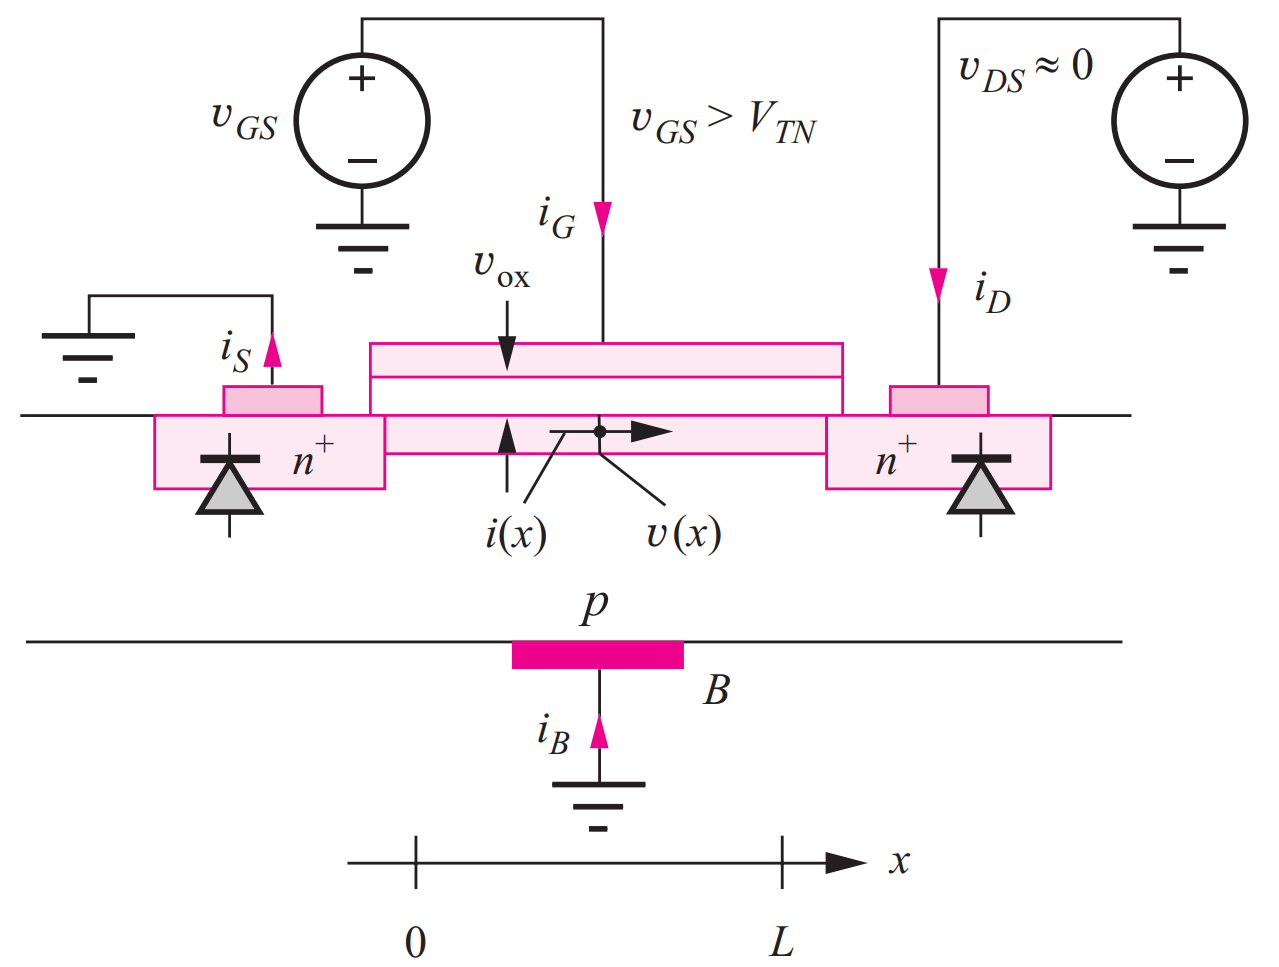
\includegraphics[width=0.4\linewidth]{img/corrente_drain.png}
    \caption{Corrente di drain}
    \label{fig:corrnte_srainnee}
\end{figure}


\paragraph{Carica nel canale}
Quanto vale la corrente di drift? Essa dipende dal campo elettrico, dalla mobilità, dalla velocità e dalla carica.

La	carica	presente	in	ogni	punto	del	canale	dipende	dalla	
tensione	sul	dielettrico,	come	in	un	condensatore.

\paragraph{Carica per unità di lunghezza}

\begin{equation}
    Q' = -WC_{ox}^{''}(v_{ox}-V_T)
\end{equation}

dove:

\begin{itemize}
    \item $C_{ox}^{''} = \frac{\varepsilon_{ox}}{T_{ox}}$, $\varepsilon_{OX}$ permittività dell'ossido e $T_{ox}$ è il suo spessore
    \item $v_{ox}(x) = V_{GS}-v_x$, $v_x$ è la tensione nel canale.
\end{itemize}

$v_{ox}\,$ deve	essere	maggiore di $V_T$ perché ci sia lo strato di inversione su tutto il canale e dunque cariche libere; $WC_{ox}^{''}$ capacità per unità di lunghezza; $v_{ox}-V_T$ tensione dell'ossido sottratta alla tensione soglia ovvero elimina il contributo degli ioni negativi fissi i quali non concorrono a creare una corrente.

La tensione sull'ossido varia lungo il canale, se in un condensatore formato da piastre metalliche ogni punto è equipotenziale, in questo caso nel semiconduttore questo non accade, quindi pure la quantità di carica non sarà costante, la differenza di potenziale sarà più alta tra source e gate a sinistra che tra drain e gate a destra Fig. \ref{fig:corrnte_srainnee}.

\newpage
\subsubsection{Corrente}
La corrente come al solito è data da:

\begin{equation}
    I(x) = Q'(x)s_x(x)\qquad \text{$s_x(x)$ velocità	delle	cariche	dovuta	al	campo	elettrico}
\end{equation}

\begin{equation}
    I(x) = -WC_{ox}^{''}(v_{ox}-V_T)(-\mu_nE_x)
\end{equation}

Ricordando il campo elettrico:

\begin{equation*}
    \vec{Ex} = -\frac{dv(x)}{dx}
\end{equation*}

Sostituendo tutto otteniamo:
\begin{equation}
    I(x) = -\mu_nWC_{ox}^{''}(V_{GS}-v_{ox}-V_T)\frac{dv(x)}{dx}
\end{equation}

Integrando lungo x:

\begin{itemize}
    \item per x = 0, v(0) = $V_S = 0$
    \item per x = L, v(L) = $V_{DS}$
    \item i(x) = $I_D$, la corrente non varia perché non ci sono altri percorsi alternativi
\end{itemize}

\begin{equation}
    \int_0^Li(x) dx = \int_0^L-\mu_nWC_{ox}^{''}(V_{GS}-v_{ox}-V_T)dv(x)
\end{equation}

Risolvendo l'integrale:

\begin{equation*}
    I_D\cdot L = \mu_nWC_{ox}^{''}(V_{GS}-V_T-\frac{V_{DS}}{2})V_{DS}
\end{equation*}
\begin{equation}
    I_D = \mu_n\frac{W}{L}C_{ox}^{''}(V_{GS}-V_T-\frac{V_{DS}}{2})V_{DS}
    \label{equazione_zona_triodo}
\end{equation}

Da notare che la corrente dipende dal rapporto di forma del transistore: $\frac{W}{L}$, in particolare quando è largo rispetto alla lunghezza. W grande corrente grande, W piccolo corrente piccola.

La corrente dipende dalla $V_{DS}$ in quanto è la "forza motrice" delle cariche e da $V_{GS}$ che mette a disposizioni gli elettroni per il passaggio di carica. Notiamo qui che la corrente dipende in modo \textbf{quadratico} con $V_{DS}$.

Valida	solo	se	la	tensione sull'ossido	è	superiore	alla soglia	VT in	ogni	punto:

\begin{itemize}
    \item $v_{ox} \geq V_T$
    \item $V_{GS} - v_{ox} \geq V_T$, $v_{ox}$ è	più	grande	al	drain
\end{itemize}

\paragraph{In particolare:}
\begin{itemize}
    \item $V_{GS} - V_{DS} \geq V_T$
    \item $V_{DS} \leq V_{GS} - V_T$
    \item $V_{GS} \geq V_{DS} + V_T$
\end{itemize}

Analizzando l'ultima disequazione: Perché  ci sia il canale, sicuramente ci deve essere una tensione $V_T$, in più aggiungiamo una tensione sul drain, ne risulta che la tensione gate-source deve essere maggiore di una VT rispetto alla tensione del drain.


\newpage
\section{Regione	lineare, ohmica	o	triodo}
Questa regione, che varia quadraticamente, viene chiamata lineare o triodo, la formula della corrente può essere riscritta in modo più compatto utilizzando la transconduttanza  ($K_N' = \mu_nC_{ox}^{''}$) che dipende dalla tecnologia (parametro tecnologico), la mobilità dei portatori dipende dal silicio e la capacità che dipende dal fattore geometrico, quale lo spessore, dell'ossido, dunque dipende da chi ve lo produce.

Talvolta nella transconduttanza viene anche inserito il rapporto tra larghezza e lunghezza: $K_N = \mu_nC_{ox}^{''}\frac{W}{L}$.

\begin{equation*}
    I_D = K_n\biggl(V_{GS}-V_T-\frac{V_{DS}}{2}\biggl)V_{DS}
\end{equation*}

\begin{equation}
    I_D = K_n\biggl((V_{GS}-V_T)V_{DS}-\frac{V_{DS}^2}{2}\biggl)
    \label{corrente_drain_formula}
\end{equation}


\paragraph{Esempio:} Calcoliamo il valore di $K_n'$ per un transistore con
\begin{itemize}
    \item $\mu_n = 500\,cm^2/Vs$ mobilità \footnote{Notiamo che la mobilità ha un valore molto più basso rispetto ai $1350\,cm^2/Vs$, questo è dovuto al fatto che le cariche si muovono sulla superficie che è a contatto con l'ossido.}
    \item $T_{os} = 25\,nm$ spessore dell'ossido 
\end{itemize}

\begin{equation*}
    K_n' = \mu_n\frac{\varepsilon_{ox}}{T_{ox}} = 500\cdot3.9\cdot8.854\cdot10^{-14}/25 = 69.1\,\mu A/V^2
\end{equation*}

\subsection{Se $V_{DS}$ è piccola}
Si chiama zona lineare perché se $V_{DS}$ è piccola la formula non compare il termine $V_{DS}^2$ e dunque il transistore si comporta come una resistenza \footnote{I = G$\cdot$V, dove G è la conduttanza $G=1/R$} (da cui anche zona ohmica) il cui valore può essere controllato da $V_{GS}$, quindi il modello diventa lineare:

\begin{equation}
    I_D = K_n(V_{GS}-V_{T})V_{DS}
\end{equation}

E per calcolare la resistenza equivalente basta fare il reciproco della conduttanza G:

\begin{equation}
    R_{on} = \frac{1}{K_n(V_{GS}-V_{T})}
\end{equation}

\begin{figure}[htbp]
    \centering
    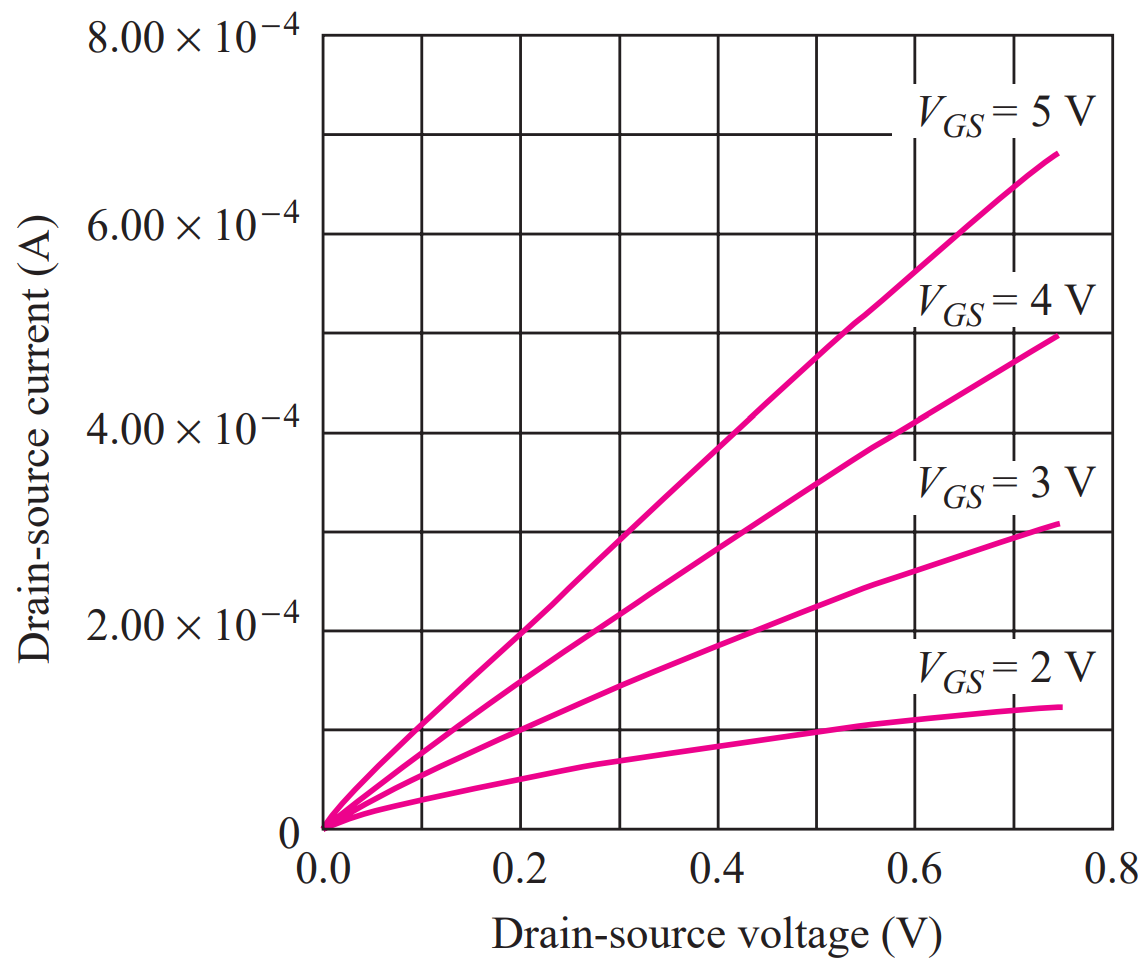
\includegraphics[width=0.4\linewidth]{img/regione_lineare.png}
    \caption{Regione lineare}
    
\end{figure}

Più si aumenta la $V_{GS}$ e più la resistenza risulterà bassa perché maggiori saranno i portatori sul canale.


\newpage
\section{Saturazione}
Il modello visto fino ad ora è valido fin tanto che:

% \begin{wrapfigure}{r}{0.6\textwidth} %this figure will be at the right
%     \centering
%     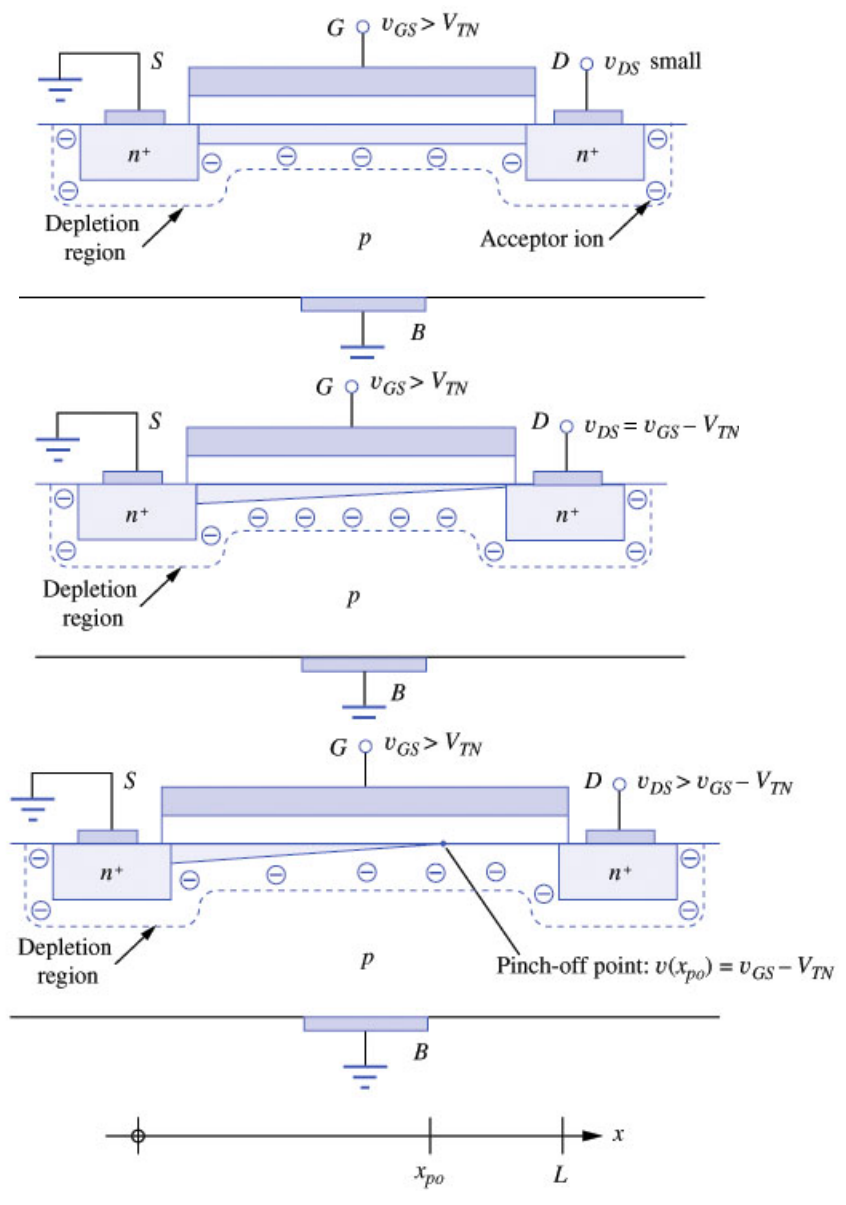
\includegraphics[width=1\linewidth]{img/image.png}
% \end{wrapfigure}


\begin{itemize}
    \item $V_{GS} \geq V_{DS} + V_{T}$
    \item La corrente $I_D$ aumenta in modo quadratico con $V_{DS}$.
\end{itemize}

\begin{figure}[htbp]
    \centering
    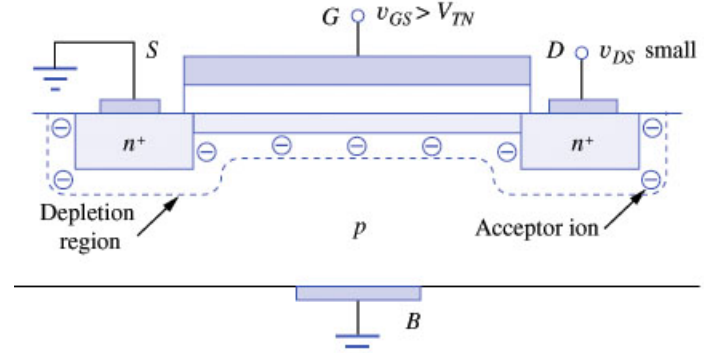
\includegraphics[width=0.45\linewidth]{img/berkley1.png}     
\end{figure}

Con l'aumento di $V_{DS}$ il canale si assottiglia verso il drain fino a scomparire per 
\begin{itemize}
    \item $V_{DS} = V_{GS} - V_{T}$
\end{itemize}

\begin{figure}[htbp]
    \centering
    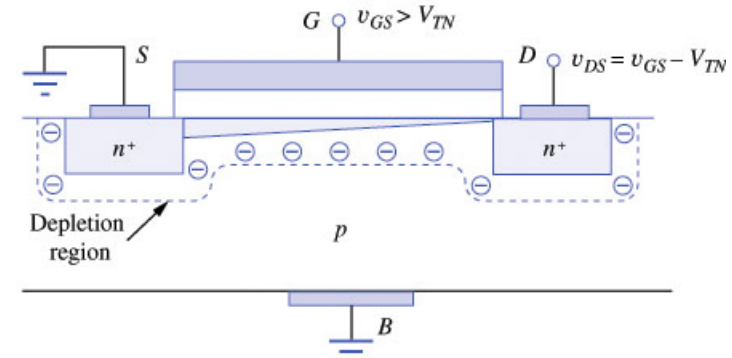
\includegraphics[width=0.45\linewidth]{img/berkley2.png}   
    
\end{figure}

Con ulteriori aumenti di $V_{DS}$ lo stato di inversione diventa nullo al drain e la corrente, non aumentando più, satura.
Quindi in prima approssimazione possiamo affermare che la corrente diventa costante, ma vedremo che non è del tutto così, leggermente aumenterà in quanto alla relazione: $E_x = -\frac{dV(x)}{dx}$, essendo che la lunghezza del canale diminuisce, aumenterà la tensione.

\begin{itemize}
    \item $V_{DS} \geq V_{GS} - V_{T}$
\end{itemize}

\begin{figure}[htbp]
    \centering
    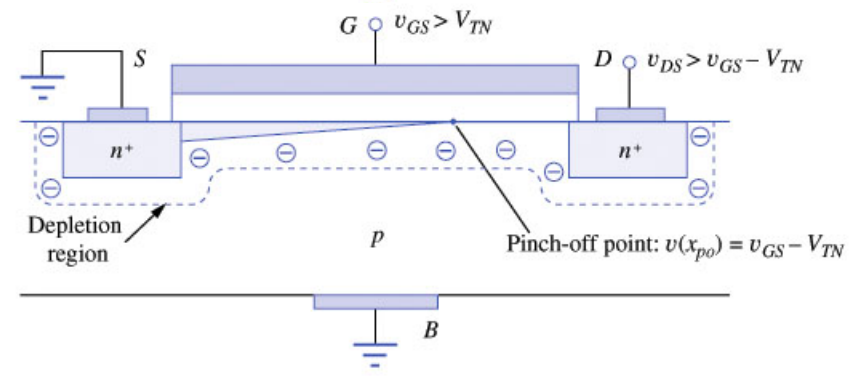
\includegraphics[width=0.45\linewidth]{img/berkley3.png}    
    
\end{figure}

\newpage
\subsection{E quanto satura?}
La corrente satura negli ultimi due casi, in particolare inizia a saturare dal valore per cui: $V_{DS} = V_{GS} - V_{T}$. E la corrente di saturazione sarà data da:

\begin{equation*}
    I_D = K_n'\frac{W}{L}\biggl(V_{GS} - V_T - \frac{V_{GS}-V_T}{2}\biggl)\big(V_{GS} - V_T\big)
\end{equation*}

\begin{equation}
    I_D = \frac{K_n'}{2}\frac{W}{L}\biggl(V_{GS} - V_T \biggl)^2
    \label{Equazione_corrente_pinch_off}
\end{equation}

Quindi vediamo subito che rispetto alla corrente di drain, Formula \ref{corrente_drain_formula}, la corrente è \textbf{indipendente} da $V_{DS}$.

La formula sopra riportata è valida per $V_{DS} \geq V_{DSAT} = V_{GS} - V_T$. La tensione $V_{DSAT}$ è chiamata tensione di \textbf{saturazione} o di \textbf{pinch-off}.

\begin{figure}[htbp]
    \centering
    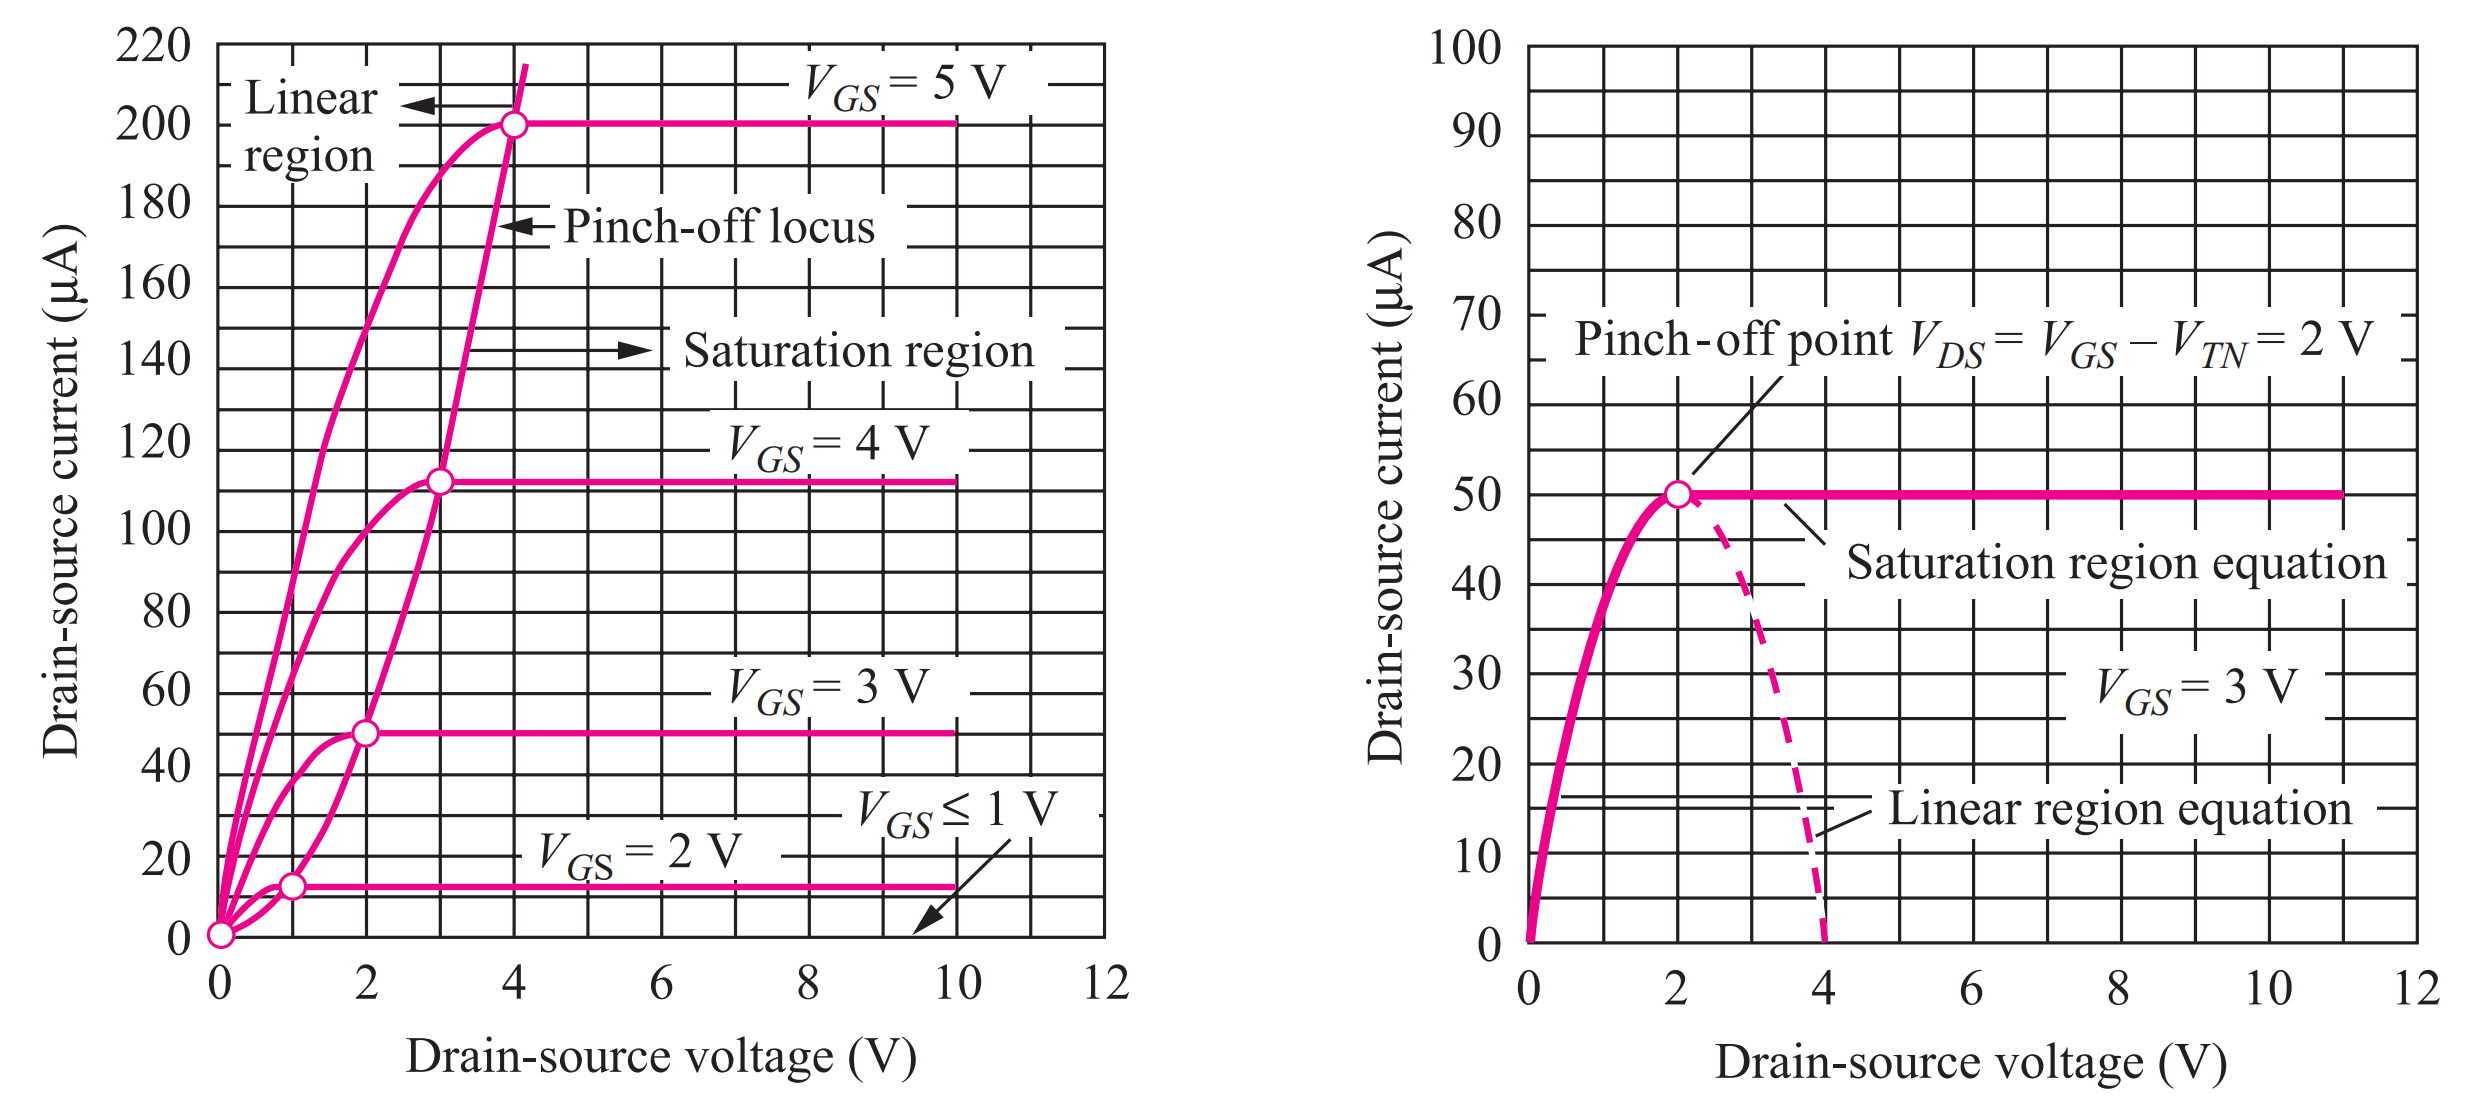
\includegraphics[width=0.9\linewidth]{img/pinch_off.png}
    \caption{Relazione corrente in funzione della tensione al drain}    
\end{figure}

 Osservando questo grafico troviamo dunque tre casi:

 \begin{itemize}
     \item $I_{DS} = 0A$
     \begin{itemize}
         \item Questo è il caso più semplice perché significa che $V_{GS} \leq V_T$
     \end{itemize}
     
    \item $V_{GS} \geq V_{DS} + V_T$
     \begin{itemize}
         \item parte del grafico che si forma una parabola rivolta verso il basso
         \item ci troviamo nella zona lineare
     \end{itemize}

     \item $ V_{DS} \geq V_{GS} - V_T$
     \begin{itemize}
         \item parte del grafico che si forma una retta
         \item ci troviamo nella zona di saturazione
     \end{itemize}     
 \end{itemize}

\paragraph{Esempio:} Supponiamo 

\begin{itemize}
    \item $V_T = 1V$
    \item $V_{GS} = 5V$
    \item $V_{DS} = 10V$
    \item $K_{n}^ = 40 \mu_A/V^2$
    \item $L = 0.35 \mu m, \quad W = 8.75 \mu m$
\end{itemize}

Per trovare \textbf{$I_D$} intanto dobbiamo capire in che regione ci troviamo utilizzando le disequazioni viste in precedenza.
In questo caso vediamo subito che siamo nella regione di saturazione e dunque possiamo applicare la relativa Formula \ref{Equazione_corrente_pinch_off} e sostituendo tutti i dati otterremmo $8 mA$.

 Da notare il rapporto di forma $W:L = 25:1$


\section{Modulazione di lunghezza di canale}
Abbiamo detto che all'aumentare di $V_{DS}$ la lunghezza del canale L effettiva diventa più piccola con la conseguenza che la corrente $I_D$ aumenta.

Normalmente nei circuiti ad alte prestazioni si vuole tenere una corrente elevata per andare più velocemente ma ovviamente ciò comporta un aumento di calore e una diminuzione della carica della batteria.

Per tener traccia di questo aumento nella formula vista in precedenza si aggiunge una costante moltiplicativa $\lambda$ chiamata parametro di modulazione di lunghezza del canale.

Normalmente $0 \leq \lambda \leq 0.2\,V^{-1}$


\begin{equation}
    I_D = \frac{K_n'}{2}\frac{W}{L}\big(V_{GS} - V_T \big)^2\big(1+\lambda V_{DS}\big)
    \label{Equazione_corrente_pinch_off_con_lambda}
\end{equation}

\begin{figure}[htbp]
    \centering
    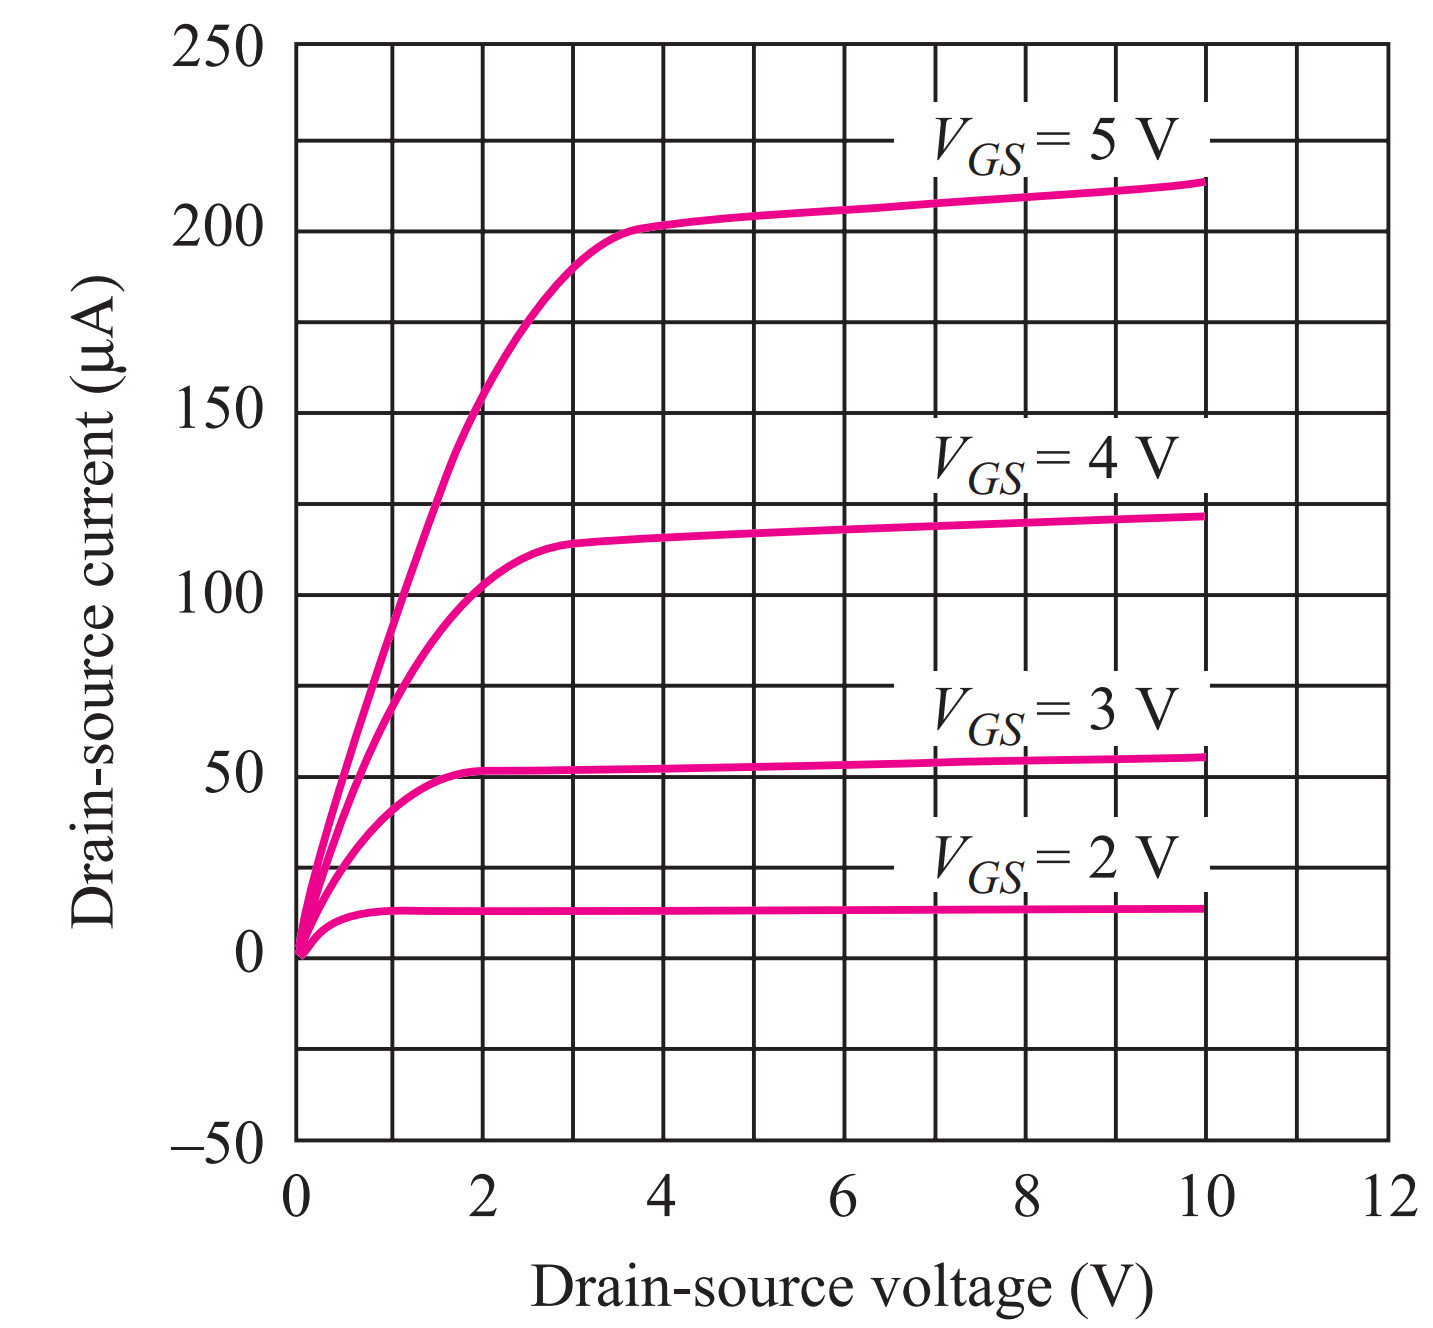
\includegraphics[width=0.4\linewidth]{img/lamda_modulazioneLungCanale.png}  
    
\end{figure}


\section{Modello matematico del transistore nMOS}

\subsubsection{Transconduttanza}

\begin{equation*}
    K_n = K_n'\frac{W}{L}\qquad\qquad K_n' = \mu_nC_{ox}''
\end{equation*}

\subsubsection{Zona triodo}
\begin{equation*}
    I_D = K_n\biggl(V_{GS}-V_{TN}-\frac{V_{DS}}{2}\biggl)V_{DS} \qquad\text{per } \qquad0\leq V_{TN} + \vds \leq \vgs
\end{equation*}

 \subsubsection{Regione di saturazione}
\begin{equation*}
    I_D = \frac{K_n}{2}\biggl(V_{GS}-V_{TN}\biggl)^2 \qquad\text{per } \qquad\vds \geq \vgs - V_{TN}
\end{equation*}

\begin{figure}[htbp]
    \centering
    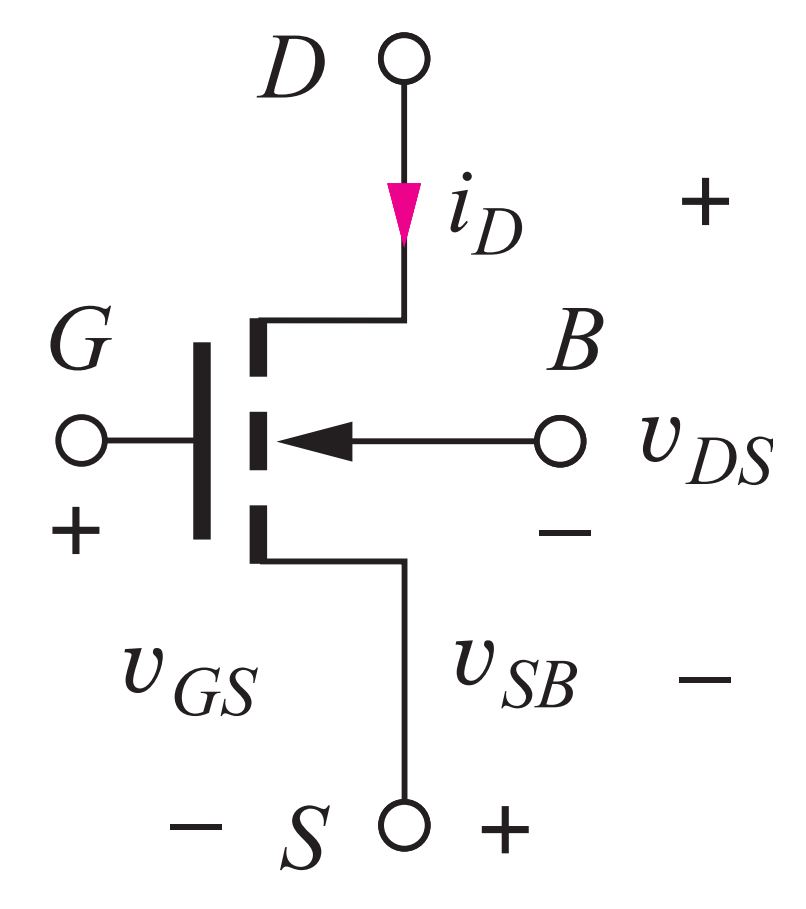
\includegraphics[width=0.2\linewidth]{img/nmossone.png}
    \caption{Transistore nMOS}
\end{figure}


\newpage
\section{Abbassare la tensione di soglia nel canale}
Arrivati a questo punto però ci potrebbe essere comodo abbassare questa tensione di soglia, il quale abbassamento farebbe in modo che il transistore possa condurre prima.

Vi sono due metodi: \textbf{Transistore	nMOS a	svuotamento} e \textbf{Effetto body}.


\section{Transistore	nMOS a	svuotamento}
Si potrebbe pensare di inserire direttamente il canale n direttamente nel substrato.

\begin{figure}[htbp]
    \centering
    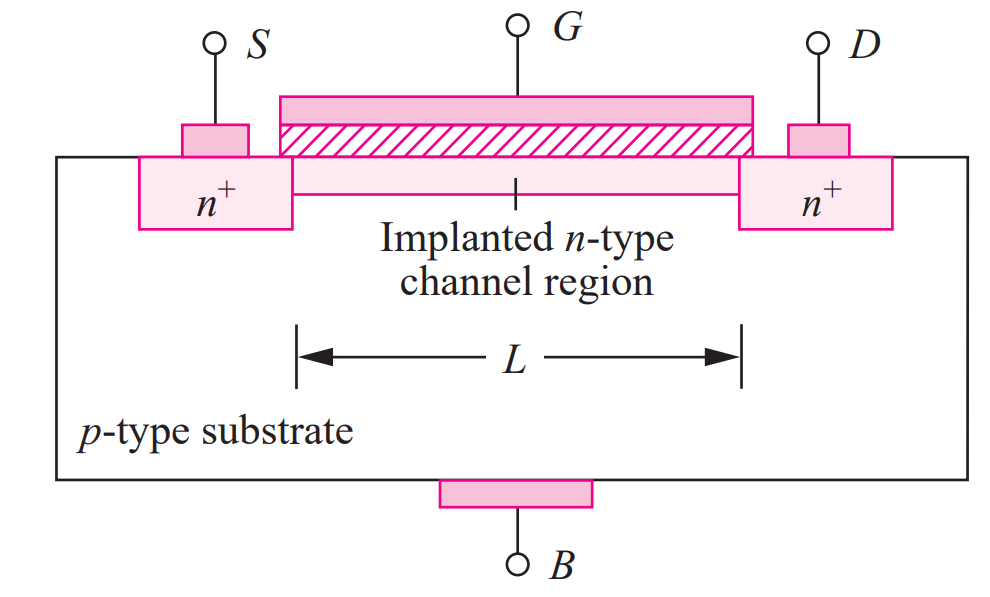
\includegraphics[width=0.4\linewidth]{img/n-type_impllanted.png}
    \caption{Transistore con canale di tipo n già inserito}
    
\end{figure}

Il canale dunque esiste già e il transistore	conduce	anche	per $\vgs = 0$, la tensione di soglia $\vt$ è  negativa, per il resto non cambia nulla.

Questo transistore prende il nome anche di transistore a \textbf{depletion mode}.


\subsection{Effetto body}

Altrimenti di potrebbe applicare una tensione al bulk $V_B$ diversa da zero per modificare la tensione di soglia

\begin{equation}
    \vt = V_{T0} + \gamma\big(\sqrt{V_{SB} + 2\phi_F} - \sqrt{2\phi_F}\big)
    \label{Equazione_effetto_body}
\end{equation}

dove
\begin{itemize}
    \item $V_{T0} $ valore di $\vt$ per $V_{SB} = 0$ , $\qquad -5\leq V_{T0} \leq 5$
    \item $\gamma $ parametro effetto body, $\qquad 0\leq \gamma \leq 3$
    \item $2\phi_F$ potenziale di superficie, $ \qquad 0.3 \leq 2\phi_F \leq 1$
\end{itemize}

\newpage
\section{Transistori pMOS}
In	modo	simmetrico,	si	può	realizzare	un	transistore	su	substrato	di	tipo	n,	con	source	e	drain	p+. Funziona tutto in maniera duale: tensioni e correnti invertire, mobilità delle lacune inferiore.

Per ottenere delle tensioni negative, non utilizzate nei dispositivi elettronici, basta mettere il source alla tensione più alta presente nel circuito, prima era a massa, e di conseguenza tutte le altre tensioni saranno inferiori o al più uguali a $V_S$.


\begin{figure}[htbp]
    \centering
    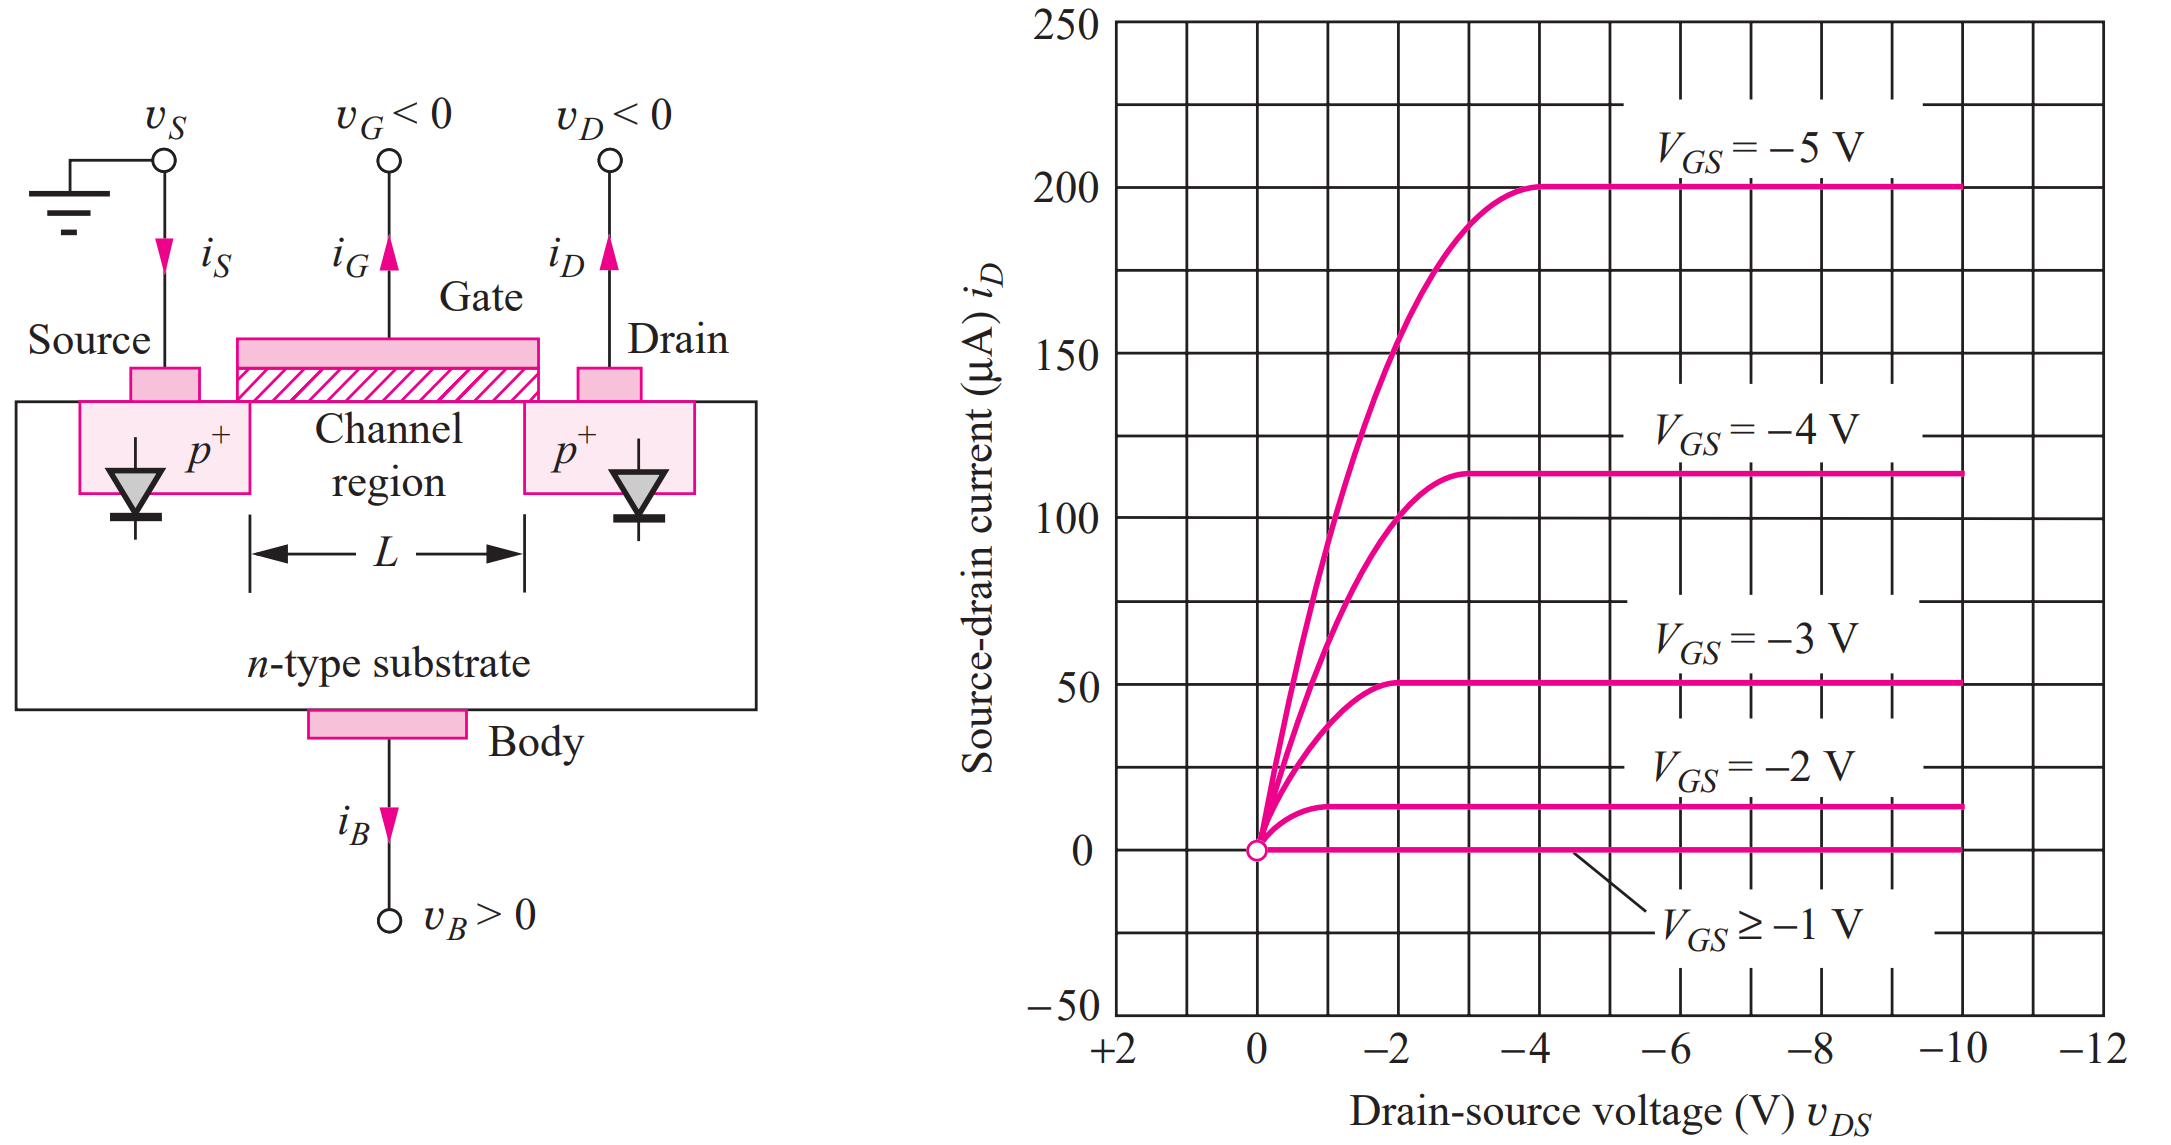
\includegraphics[width=0.8\linewidth]{img/pMOS.png}
    \caption{Transistore pMOS}    
\end{figure}

\section{Modello matematico del pMOS}

\subsubsection{Transconduttanza}

\begin{equation*}
    K_p = K_p'\frac{W}{L}\qquad\qquad K_p' = \mu_pC_{ox}''
\end{equation*}

\subsubsection{Zona triodo}
\begin{equation*}
    I_D = K_p\biggl(V_{GS}-V_{TP}-\frac{V_{DS}}{2}\biggl)V_{DS} \qquad\text{per } \qquad0\leq |\vds|\leq |\vgs - V_{TP}|
\end{equation*}

 \subsubsection{Regione di saturazione}
\begin{equation*}
    I_D = \frac{K_p}{2}\biggl(V_{GS}-V_{TP}\biggl)^2 \qquad\text{per } \qquad |\vds| \geq |\vgs - V_{TP}|
\end{equation*}

\begin{figure}[htbp]
    \centering
    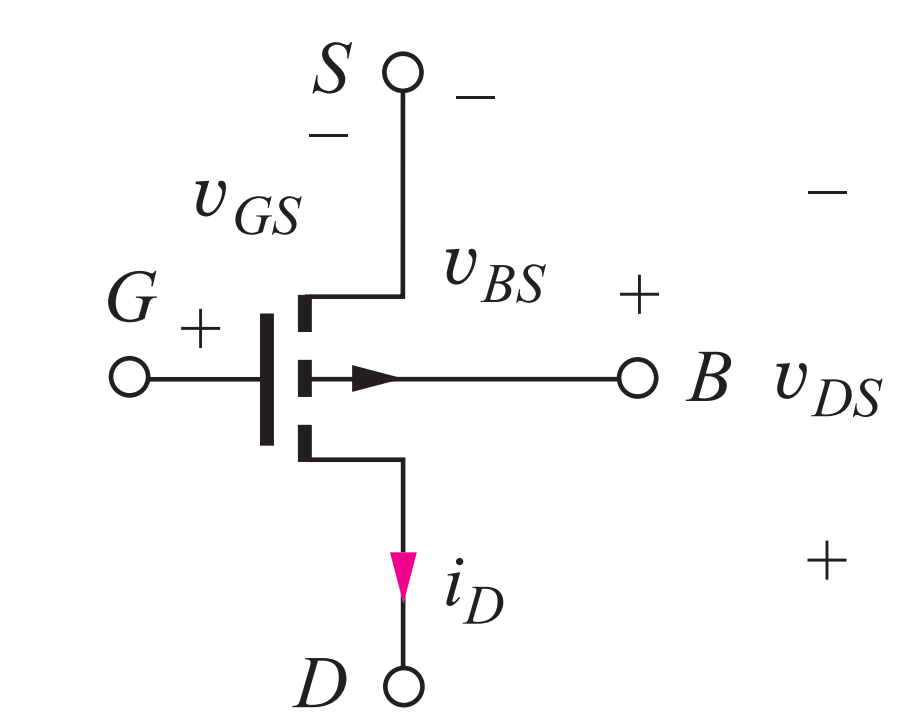
\includegraphics[width=0.27\linewidth]{img/p_mos.png}
    \caption{Transistore pMOS}    
\end{figure}


\section{Riassunto}

Nel transistore MOSFET troviamo quattro terminali: 

\begin{itemize}
    \centering
    \item[] Gate \qquad \qquad Source \qquad \qquad Drain \qquad \qquad Body
\end{itemize}

e tre zone di funzionamento:

\begin{itemize}
    \item[] \textbf{Cut-off}: se $\vgs$ è sotto la tensione di voglia $\vt$, ciò non fa scorrere corrente tra $I_D$ tra drain e source
    \item[] \textbf{Triodo}: se $\vgs$ è sopra la tensione di soglia $\vt$ lungo tutto il canale, la corrente $I_D $ tra	drain	e	source	dipende	da	$\vgs$ e	da	$\vds$ secondo	la	legge	quadratica :
    \begin{itemize}
        \item[] \begin{equation*}
            I_D = K_n\biggl(V_{GS}-V_T-\frac{V_{DS}}{2}\biggl)V_{DS}\qquad \text{per} \qquad \vt \leq \vgs \geq \vds + \vt
        \end{equation*}
    \end{itemize}

    \item[] \textbf{Saturazione} se $\vgs$ è	sopra	la	tensione	di	soglia $\vt$ per	parte	
    del	canale,	la	corrente $I_D$ tra	drain	e	source	non	dipende	da $\vds$ e dipende da $\vgs$ secondo una legge quadratica:
    \begin{itemize}
        \item[] \begin{equation*}
                I_D = \frac{K_n}{2}\biggl(V_{GS} - V_T \biggl)^2\qquad \text{per} \qquad \vgs \leq \vds + \vt
        \end{equation*}
    \end{itemize}

\end{itemize}

\begin{figure}[htbp]
    \centering
    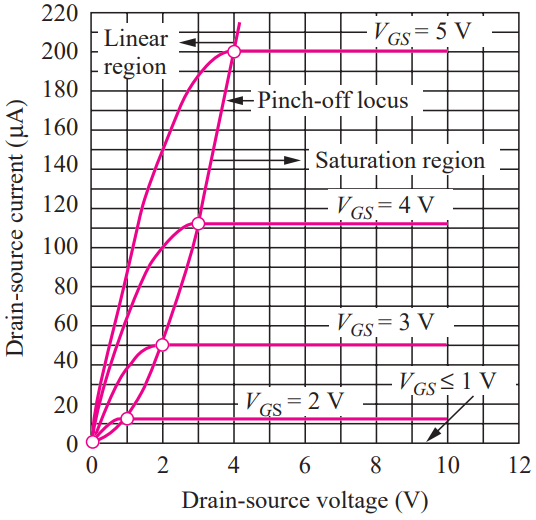
\includegraphics[width=0.45\linewidth]{img/recap.png}
    \caption{Caratteristica I-V}
    
\end{figure}

\newpage
\section{Modello di analisi}
Occorre	stabilire	la	regione	di	funzionamento	del	transistore	in	modo	da	applicare	la	formula	giusta. Se	difficile	da	dire	a	priori,	si	fanno	delle	ipotesi	e	poi	si	verifica	
che	i	risultati	siano	consistenti	con	le	ipotesi	(come	già	fatto	
per	i	diodi).

Spesso	si	faranno	delle	semplificazioni,	considerando	solo	il	
punto	di	inizio	e	di	fine	di	un	transitorio,	per	evitare	di	dover	
integrare	lungo	tutta	la	caratteristica.

\subsubsection{Circuiti digitali e amplificatori}

Per	circuiti	digitali	si	lavora	in	cut-off	(interruttore	aperto)	o	in	
regione	lineare	(interruttore	chiuso)

\subsubsection{Amplificatori}

Per	amplificatori	si	lavora	in	regione	di	saturazione	(generatore	
di	corrente	costante,	controllata	dalla	tensione	di	ingresso)

\paragraph{}
Bisogna fare attenzione che la $\vds$ dipende dal resto del circuito, infatti non 	è	imposta	direttamente	da	un
generatore	di	tensione ma dipende	dalla	corrente	di	drain.

\subsection{Calcolo con la retta di calcolo}

Dato il seguente circuito, formato da un singolo transistore con source a massa e gate e drain collegato ad un generatore di tensione.

Assumendo $\vt = 1V$ e $K_n = 220 \mu A/V^2$, trovare la corrente e la tensione tra drain e source.

$\vt$ è possibile trovarla facilmente. Basta mettersi in un punto di pinch-off e fare la differenza tra $\vgs$ e $\vds$.
\paragraph{}

\begin{figure}[htbp]
    \centering
    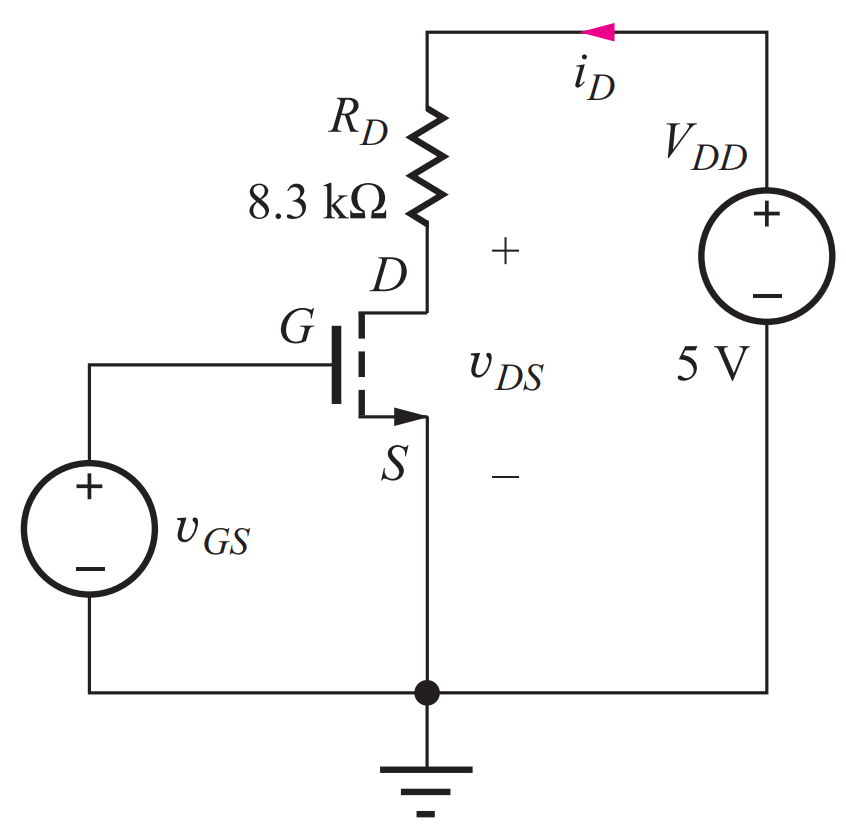
\includegraphics[width=0.3\linewidth]{img/calcolo_retta_carico.png}
    \caption{Circuito}    
\end{figure}

Per prima cosa dobbiamo trovare la retta di carico, ed utilizziamo l'equazione alla maglia del circuito a destra.

\begin{equation*}
    V_{DD} = I_DR + V_{DS}
\end{equation*}

Trovando che se la corrente è zero allora $\vds = \vgs$, e per trovare la massima corrente applicheremo la legge di Ohm tra la tensione $V_{DD}$ e la resistenza R.

Fatto ciò possiamo tracciare la retta di carico:

\begin{figure}[htbp]
    \centering
    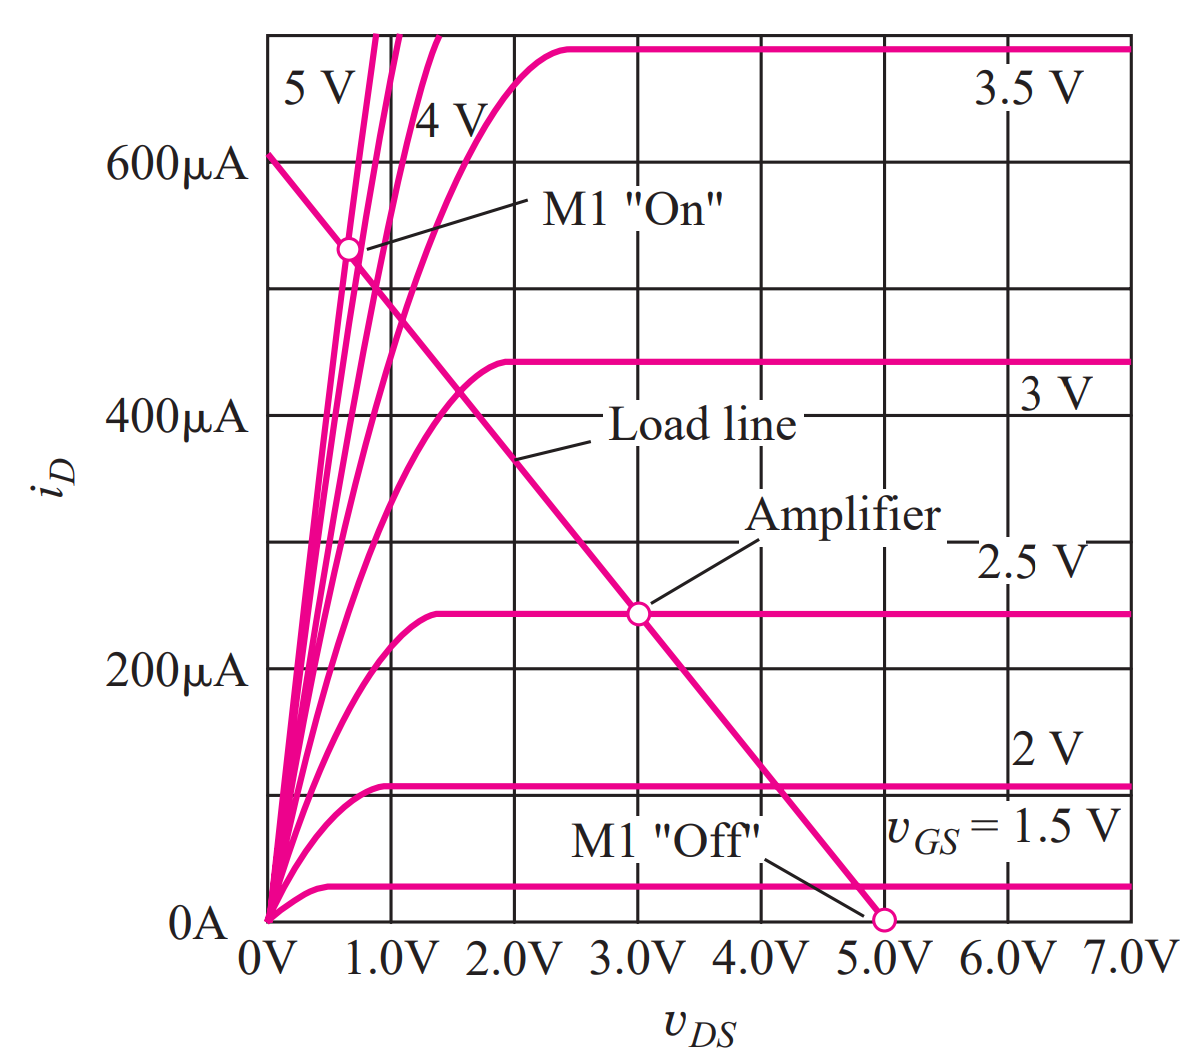
\includegraphics[width=0.5\linewidth]{img/retta_carico_es.png}    
\end{figure}

\newpage

Ora vediamo a vari valori di $\vgs$ come si comporta.

\subsubsection{$\vgs \leq \vt$}

In questo caso vediamo che la corrente di drain è zero pure la corrente nella resistenza è zero

\paragraph{Troviamo M1}
Supponiamo ora di essere nella regione lineare e che $\vgs  = V_{DD}$, e che la tensione sia tutta sulla resistenza, dunque che $\vds$ sia piccola.  

Utilizzando la Formula \ref{equazione_zona_triodo} e l'equazione della retta di calcolo vista prima, mettendole a sistema possiamo trovare $\vds$ e $I_D$.

\begin{equation*}
    \vdd = K_n\biggl(\vgs - \vt - \frac{\vds}{2}\biggl)\vds R + \vds
\end{equation*}
\begin{equation*}
    \frac{K_nR}{2}\vds^2 - \big[1+K_nR(\vgs - \vt)\big]\vds + \vdd = 0
\end{equation*}
\begin{equation*}
    \vds = \frac{1+K_nR(\vgs - \vt)\pm \sqrt{\Big(1+K_nR(\vgs - \vt)\Big)^2 - 2K_nR\vdd} }{K_nR}
\end{equation*}
\begin{equation*}
    \vds = 0.65 V\qquad\qquad\qquad I_D = 525 \mu A
\end{equation*}

\subsubsection{Supponiamo di essere in saturazione}

Con $\vgs = 2.5V$ notiamo immediatamente dal grafico che ci troviamo in satura saturazione, proviamo dunque a calcolare come prima tensione e corrente, utilizzando sempre l'equazione della retta di calcolo e anche la Formula \ref{Equazione_corrente_pinch_off}.

\begin{equation*}
    \vdd = \frac{K_n}{2}(\vgs-\vt)^2R + \vds
\end{equation*}

\begin{equation}
    \vds = \vdd - \frac{K_n}{2}(\vgs-\vt)^2R
    \label{equazione_vds}
\end{equation}

\begin{equation*}
    \vds = 2.95 V\qquad\qquad\qquad I_D = 247.5\mu A
\end{equation*}

In questa zona il transistore ha una corrente costante e dunque si comporta come un generatore di corrente, e il valore della corrente lo controlliamo con la $\vgs$. Per piccole variazioni di $\vgs$, questo comporta il muoversi sulla retta di carico, causano grosse variazioni di $\vds$, funziona come un amplificatore.

\newpage
\subsection{Come determinare l'uscita $\vds$ in funzione dell'ingresso $\vgs$}

Vorremmo capire che relazione ci sia tra $\vds$ e $\vgs$, sicuramente dovremo vedere tutte le zone di funzionamento.

\subsubsection{Zona di Cut-off}

Partendo da $\vgs$ piccola, fintantoché questa è inferiore a $\vt$, corrente nel drain non ne scorre, non c'è caduta di potenziale sulla resistenza e l'uscita è 5V.

Questa zona infatti risulterà essere piatta.

\begin{figure}[htbp]
    \centering
    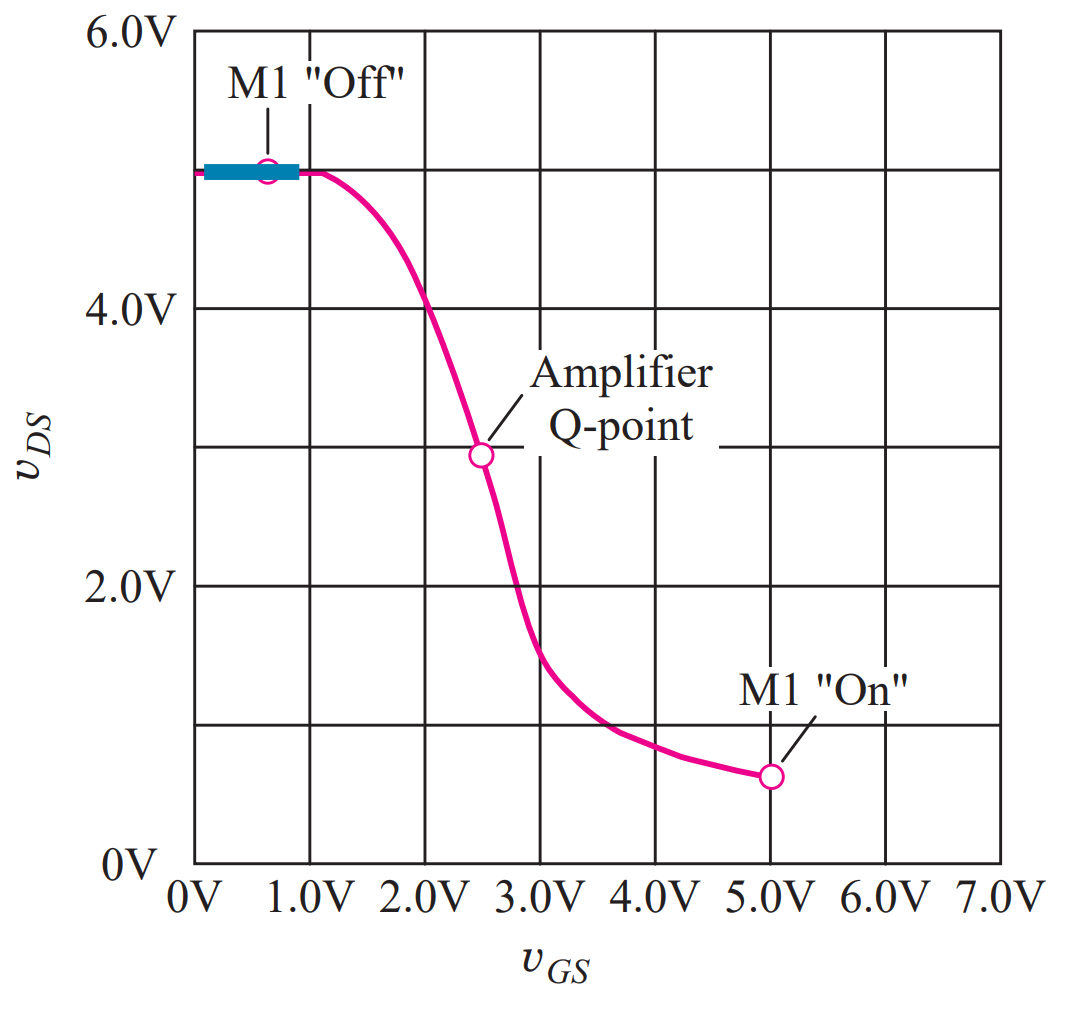
\includegraphics[width=0.4\linewidth]{img/IO_off.png}
    \caption{$\vgs < \vt$}    
\end{figure}

\subsubsection{Zona di amplificazione/saturazione}

Per ricavare la curva in questo caso basta assegnare dei valori a $\vgs$. Prendendo le equazioni della corrente e della retta di carico come fatto prima per ottenere la Formula \ref{equazione_vds} e sostituendoci $\vgs = \vds + \vt $ per trovare la zona di confine.

Questo vale fino a che $\vgs \leq \vds + \vt$

\begin{equation*}
    \vds = \frac{-2\pm \sqrt{4 + 8K_nRV_{DD}}}{2K_nR}
\end{equation*}

Una soluzione verrà negativa che ovviamente va scartata perché non c'è nessuna tensione negativa in questo circuito.

\begin{figure}[htbp]
    \centering
    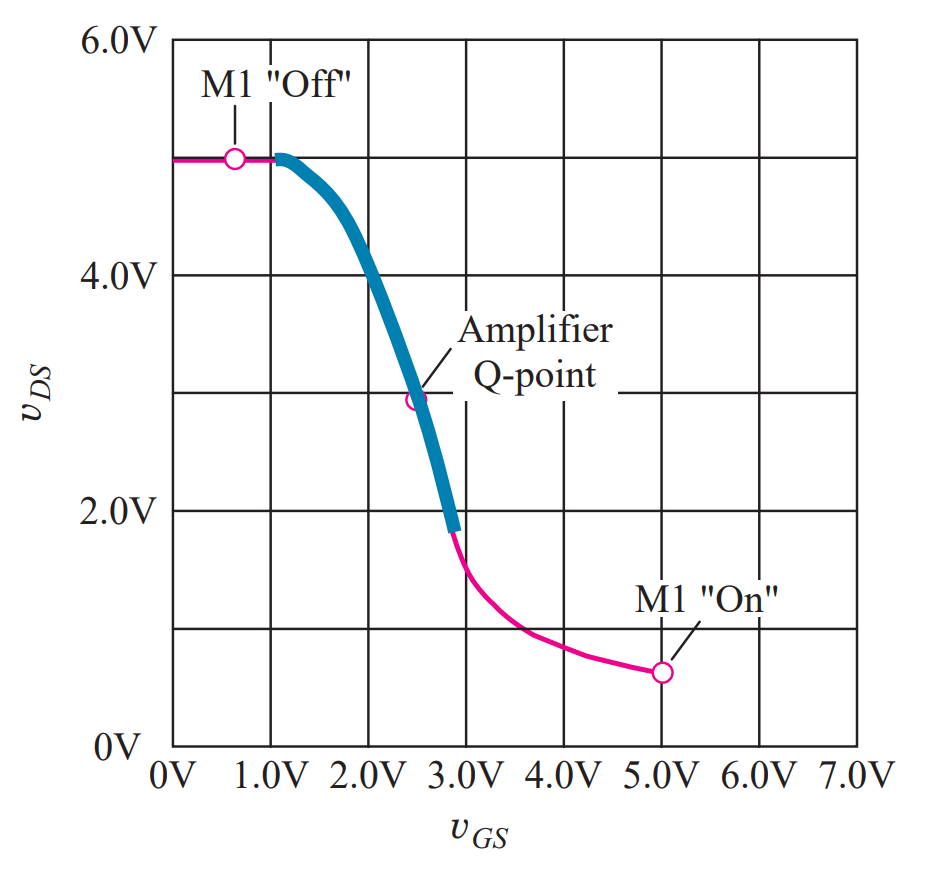
\includegraphics[width=0.4\linewidth]{img/IO_ampl.png}
    \caption{$\vgs \leq \vds + \vt$}    
\end{figure}


\subsubsection{Zona di triodo}

Successivamente per $\vgs > \vds + \vt$ il transistore funziona in zona trodo.

\begin{equation*}
    V_{DS} = \frac{1+K_nR(\vgs - \vt ) \pm \sqrt{(1 + K_nR(\vgs - \vt))^2 - 2K_nR\vdd}  }{K_nR}
\end{equation*}

\begin{figure}[htbp]
    \centering
    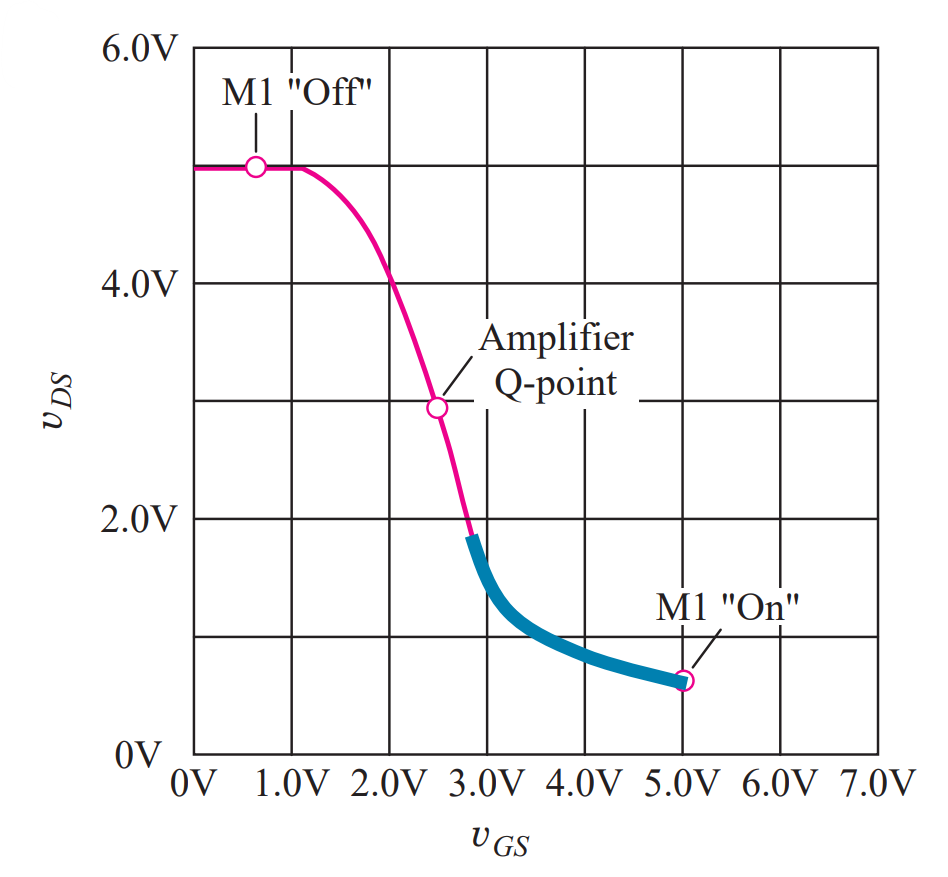
\includegraphics[width=0.4\linewidth]{img/IO_triodo.png}
    \caption{$\vgs > \vds + \vt$}    
\end{figure}

Si può vedere che se l'ingresso è basso l'uscita è alta; se l'ingresso è alto l'uscita è bassa, anche perchè se fosse l'ingresso ad un altro transistore sarebbe sotto soglia (1V). Si comporta come invertitore logico.

Nella zona intermedia si comporta in modo differente: un piccolo cambiamento di $\vgs$, l'ingresso, comporta un grande cambiamento per l'uscita $\vds$. La derivata in valore assoluto è maggiore di 1.


\newpage
\section{Saturazione di velocità}
Come accennato in precedenza, all'aumentare del campo elettrico  i portatori raggiungeranno un limite di velocità, oltre ($\vec{E} > 10^5\,V/cm$) non aumentano più.

In maniera approssimata possiamo dire che $\vec{E} = \frac{\vds}{L}$, dunque aumentiamo il campo elettrico aumenta la corrente (perché aumenta la velocità dei portatori). Se la velocità satura, aumentando il campo elettrico ma la velocità non aumenta e nemmeno la corrente la quale diventa costante.
\paragraph{}
Una saturazione di velocità porta inevitabilmente ad una saturazione di corrente, non dovuta al fatto che non vi è più inversione ma è dovuta al fatto che i portatori non possono andare più velocemente. Si potrebbe arrivare prima in saturazione di velocità rispetto alla saturazione di pinch-off, questo dipende dalla lunghezza del canale.

Normalmente con le tecnologie moderne, siamo sempre in saturazione di velocità, e soprattutto vogliamo correnti elevate.

\paragraph{}

Dunque ad un	certo	punto,	pur	aumentando	$\vds$ e	quindi	il	campo elettrico	$\vec{E}$,	la	velocità	non	aumenta	più.

Supponiamo che la saturazione si raggiunga per $\vds = V_{SAT} = \vec{E}\cdot L$, la corrente non aumenta più in funzione a $\vds$.

\paragraph{Nota:}
Non	confondete	la	\textbf{regione	di	saturazione} con	la	\textbf{saturazione	di	velocità}.	
Si	può	avere	saturazione	di	velocità	in	zona	triodo,	o	non	avere	
saturazione	di	velocità	in	regione	di	saturazione!

Se	siamo	in	regione	di	saturazione	con	\textbf{saturazione	di	velocità},	la	
corrente	cresce	linearmente	con $\vgs$,	invece	che	quadraticamente!

\paragraph{Esempio: } si consideri $L = 1\mu m$, $100 nm$, $22 nm$, $5nm$. Troviamo a che valore di $\vds$ causa la saturazione di velocità:

\begin{itemize}
    \item[] $V_{SAT} = 10^{-4}\cdot10^5 = 10 V$
    \item[] $V_{SAT} = 10^{-5}\cdot10^5 = 1 V$
    \item[] $V_{SAT} = 22\cdot10^{-6}\cdot10^5 = 0.22 V$
    \item[] $V_{SAT} = 5\cdot10^{-7}\cdot10^5 = 0.05 V$
\end{itemize}

Se prendiamo in considerazione il secondo caso, è normale usare 1V nei circuiti, ma talvolta potremmo avere tensioni più alte come 1.8V e a quel punto saremo in saturazione di velocità.

Con $22nm$ siamo praticamente sempre in saturazione di velocità perché la tensione di alimentazione non è ancora arrivata ad essere 0.22V, ma non potrà mai essere sotto a 0.6 V perché il transistore ha una tensione di soglia e se si scende sotto ad essa non si può proprio accendere. Per ovviare a questo ci sono altri metodi.


\subsubsection{Saturazione di velocità}
La zona di saturazione è un limite che sotto al quale possiamo essere o in zona \textbf{triodo} o in nella regione di \textbf{pinch-off}.
L'espressione singola che riassume il tutto e la segiente:

\begin{equation}
    I_D = K_n\biggl(\vgs - \vt -\frac{V_{MIN}}{2}\biggl)V_{MIN}(1-\lambda\vds)
\end{equation}

dove $V_{MIN}:$

\begin{equation*}
    V_{MIN} = min((\vgs - \vt ), \vds, V_{SAT})
\end{equation*}

quindi il minimo tra, in ordine, saturazione, triodo e saturazione di velocità.

\begin{figure}[htbp]
    \centering
    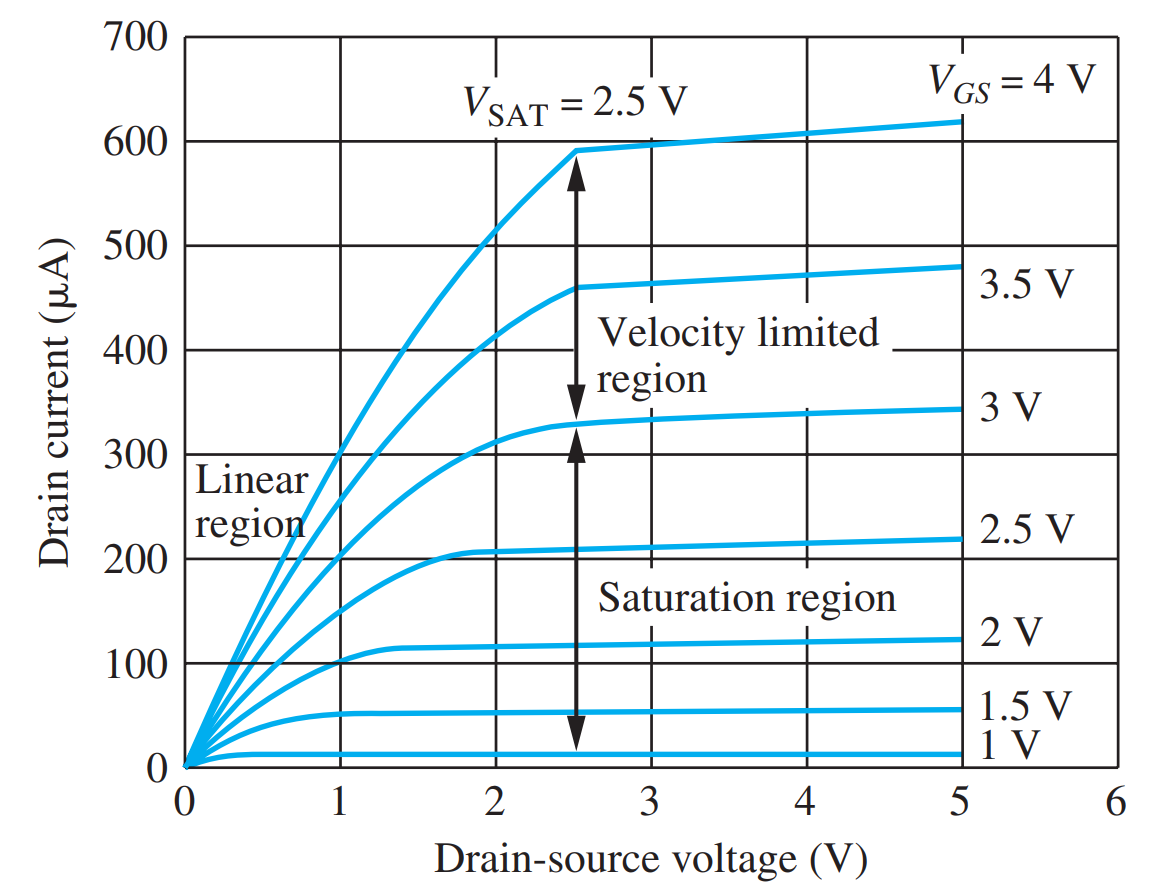
\includegraphics[width=0.5\linewidth]{img/v_sat.png}
    \caption{Regione di saturazione}    
\end{figure}

\newpage
\subsection{Conduzione sotto soglia}
Abbiamo detto che per $\vgs < \vt$ la	corrente	di	drain	è	nulla. Ma	anche questa è	una	approssimazione,	infatti ci	sono	comunque	dei	portatori		e	ci	sono	le	correnti	inverse	dei	diodi. 

Se $V_{DS} > 0$ scorre una debole corrente, più	la	tensione	di	soglia	è	bassa,	più	è	alta	la	corrente	sotto	
soglia. Ciò può	diventare	significativa	quando	ci sono	miliardi	di	dispositivi!

\begin{figure}[htbp]
    \centering
    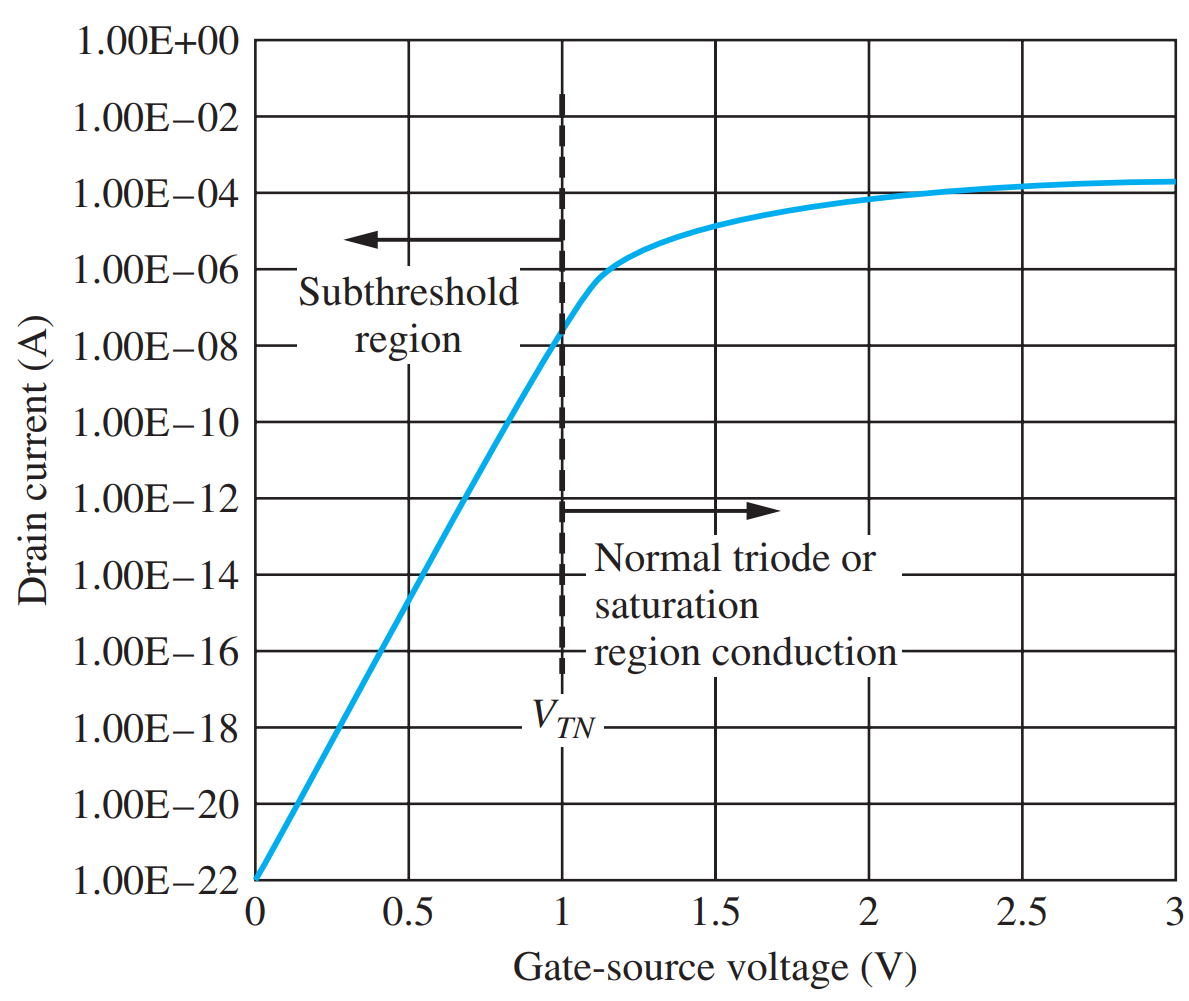
\includegraphics[width=0.5\linewidth]{img/corrente_sotto_soglia.png}
    \caption{Corrente sotto soglia, con $V_{DS}$ fissata}
    
\end{figure}


Inoltre tanto più bassa è la soglia del dispositivo, tanto più alta è la corrente sotto soglia. Sarebbe bello fare dei transistori con tensione di soglia molto piccola perché diminuirebbe l'assorbimento di potenza, ma ciò non è possibile perché conduce.

Alcuni circuiti basano il loro funzionamento proprio sul fatto che vi è questa corrente sotto soglia, ma ciò comporta che questi circuiti vadano bene se vogliamo costruite dispositivi non preformanti: il sensore di temperatura.
\paragraph{}
Ad alte prestazioni questa corrente sotto soglia comporta che il dispositivo consuma anche quando sta fermo, idealmente una porta consuma quando si deve scaricare e caricare, non quando sta ferma. Questo consumo non possiamo evitarlo il quale si attesta sull'ordine dei $mA$.






